\documentclass[sigconf,screen,balance=false]{acmart}

\newcommand{\asplossubmissionnumber}{399}

\usepackage[normalem]{ulem}

\usepackage[ruled,vlined]{algorithm2e}
% \usepackage{algpseudocode}
% \usepackage{balance}
\usepackage{amssymb}
% \usepackage{mathrsfs}
% \usepackage{microtype}
\usepackage{listings}
\usepackage{graphicx}
\usepackage{xspace}
\usepackage{booktabs}
\usepackage{subcaption}
\usepackage{minted}
\usepackage{enumitem}

% \citestyle{acmauthoryear}
% Comment macros
\newcommand{\milind}[1]{\textcolor{blue}{\sl{\bf Milind:} #1}}
\newcommand{\raghav}[1]{\textcolor{orange}{\sl{\bf Raghav:} #1}}
% \newcommand{\raghav}[1]{}
\newcommand{\kabir}[1]{\textcolor{magenta}{\sl{\bf Ben:} #1}}

\newcommand{\system}{\text{Coyote}\xspace}

\newcommand\samplefrom{\mathrel{\reflectbox{$\leadsto$}}}
% \newcommand{\Description}[1]{}
% \newcommand{\citet}[1]{\cite{#1}}

\title{Coyote: A Compiler for Vectorizing Encrypted Arithmetic Circuits}

\author{Raghav Malik}
\affiliation{
    \department{School of Electrical and Computer Engineering}
    \institution{Purdue University}
    \city{West Lafayette}
    \state{IN}
    \country{USA}}
\email{malik22@purdue.edu}

\author{Kabir Sheth}
\affiliation{
    \department{School of Electrical and Computer Engineering}
    \institution{Purdue University}
    \city{West Lafayette}
    \state{IN}
    \country{USA}}
\email{kdsheth@purdue.edu}

\author{Milind Kulkarni}
\affiliation{
    \department{School of Electrical and Computer Engineering}
    \institution{Purdue University}
    \city{West Lafayette}
    \state{IN}
    \country{USA}}
\email{milind@purdue.edu}
%%% The following is specific to ASPLOS '23 and the paper
%%% 'Coyote: A Compiler for Vectorizing Encrypted Arithmetic Circuits'
%%% by Raghav Malik, Kabir Sheth, and Milind Kulkarni.
%%%
\setcopyright{rightsretained}
\acmPrice{}
\acmDOI{10.1145/3582016.3582057}
\acmYear{2023}
\copyrightyear{2023}
\acmSubmissionID{asplosc23main-p399-p}
\acmISBN{978-1-4503-9918-0/23/03}
\acmConference[ASPLOS '23]{Proceedings of the 28th ACM International Conference on Architectural Support for Programming Languages and Operating Systems, Volume 3}{March 25--29, 2023}{Vancouver, BC, Canada}
\acmBooktitle{Proceedings of the 28th ACM International Conference on Architectural Support for Programming Languages and Operating Systems, Volume 3 (ASPLOS '23), March 25--29, 2023, Vancouver, BC, Canada}
\received{2022-10-20}
\received[accepted]{2023-01-19}
\begin{document}
\begin{abstract}

Fully Homomorphic Encryption (FHE) is a scheme that allows a computational circuit to operate on encrypted data and produce a result that, when decrypted, yields the result of the unencrypted computation. While FHE enables privacy-preserving computation, it is extremely slow. However, the mathematical formulation of FHE supports a SIMD-like execution style, and hence recent work has turned to vectorization to recover some of the missing performance. Unfortunately, these vectorization approaches do not work well for arbitrary computations: they do not account for the high cost of {\em rotating} vector operands to allow data to be used in multiple operations. Hence, the cost of rotation can outweigh the benefits of vectorization.

This paper presents \system, a new approach to vectorizing encrypted circuits that specifically aims to optimize the use of rotations. It vectorizes entire subcircuits at once to eliminate rotations within those subcircuits. It then attempts ``lines up'' operations between subcircuits using a minimal number of rotations. \system uses a careful encoding of the {\em lane placement} problem that allows a solver to identify good rotations without having to explore an impractically large search space. This paper shows that \system is effective at vectorizing computational kernels while minimizing rotation, finding efficient vector schedules and smart rotation schemes to achieve substantial speedups.

\end{abstract}

\begin{CCSXML}
    <ccs2012>
       <concept>
           <concept_id>10002978.10002979</concept_id>
           <concept_desc>Security and privacy~Cryptography</concept_desc>
           <concept_significance>500</concept_significance>
           </concept>
       <concept>
           <concept_id>10011007.10011006.10011041</concept_id>
           <concept_desc>Software and its engineering~Compilers</concept_desc>
           <concept_significance>500</concept_significance>
           </concept>
       <concept>
           <concept_id>10011007.10011006.10011050.10011017</concept_id>
           <concept_desc>Software and its engineering~Domain specific languages</concept_desc>
           <concept_significance>500</concept_significance>
           </concept>
       <concept>
           <concept_id>10002978.10003022</concept_id>
           <concept_desc>Security and privacy~Software and application security</concept_desc>
           <concept_significance>300</concept_significance>
           </concept>
     </ccs2012>
\end{CCSXML}
    
\ccsdesc[500]{Security and privacy~Cryptography}
\ccsdesc[500]{Software and its engineering~Compilers}
\ccsdesc[500]{Software and its engineering~Domain specific languages}
\ccsdesc[300]{Security and privacy~Software and application security}

\keywords{Homomorphic Encryption, Arithmetic Circuits, Vectorization}

\maketitle

\section{Introduction}\label{sec:intro}
\begin{itemize}
    \item Motivation
    \item Results
    \item Contributions
    \item Layout of the paper
\end{itemize}

%% Motivation
% What's the big picture problem?
Fully Homomorphic Encryption (FHE) refers to any encryption scheme that allows for homomorphically adding and multiplying ciphertexts, so that the sum of the encryptions of two integers is an encryption of their sum, and similarly the product of the encryptions of two integers is an encryption of their product.
While FHE is an incredibly powerful technique for carrying out privacy-preserving computations on encrypted data, it has a major downside: its slow.
Homomorphic computations over ciphertexts are often orders of magnitude slower than their plaintext counterparts.
\raghav{I wonder if reviewers will read this and think ``hmm there was a PLDI paper last year that said the same thing''}
Many FHE cryptosystems support packing large numbers of ciphertexts into {\em ciphertext vectors}, essentially compensating for the inherent slowness of FHE by enabling SIMD-style computation.
To properly take advantage of ciphertext packing, we need a compiler that can vectorize arbitrary FHE programs.

% Who has tried to solve this problem before?
Vectorizing compilers for FHE are nothing new \cite{CHET, Porcupine}.

%% Contributions

%% Results

\subsection{Related Work} % limit this to basically a couple sentences, not a whole subsection
% "These are approaches people have tried that don't work"
\subsubsection{Vectorizing FHE} \raghav{CHET and Porcupine: not general}
\subsubsection{SLP} \raghav{Assumes shuffling data between lanes is cheap}
\section{Background}\label{sec:background}
\subsection{Fully Homomorphic Encryption}
Fully Homomorphic Encryption (FHE) refers to any encryption scheme with the property that ciphertexts can be added and multiplied, and these operations commute with the encryption and decryption functions. \cite{Gentry}
In other words, encrypting inputs, computing over them, then decrypting the result is equivalent to computing over the un-encrypted inputs. FHE is hence useful for computing on encrypted data, improving privacy in situations such as computation offloading.
Since addition and multiplication are complete, FHE can theoretically be used to realize arbitrary functions on encrypted data.

The Brakerski/Fan-Vercauteren (BFV) \cite{BFV} cryptosystem, which is the particular FHE scheme that we use in this paper, is based on the Ring Learning With Errors (RLWE) problem.
Ciphertexts in BFV are represented as high degree polynomials with an ``error term'', which is a small amount of noise added to the polynomial to make the scheme ``CPA-secure'' (in other words, the same plaintext will not encrypt to the same ciphertext each time).
\subsubsection{Limitations}
% very slow
While FHE is an attractive approach to performing privacy-preserving computation, it does present a few challenges.
The first is that the polynomial encoding of ciphertexts incurs a huge overhead for any secure computation.
To achieve a reasonable degree of security, the polynomials need to be quite large, so a single primitive ciphertext operation like an add or a multiply gets translated into notoriously expensive polynomial math.
This means that all but the smallest FHE applications are often too slow to be run in a practical amount of time.

% multiplicative depth
Another main challenge of FHE computation is related to the noise added to ciphertexts.
When setting up an FHE computation, the encryption parameters used determine a safe {\em noise margin} for ciphertexts, which describes the level of noise above which ciphertexts can no longer be decrypted.
Freshly encrypted ciphertexts are well below this margin, but multiplying two ciphertexts increases the amount of noise present in the result.
BFV does support {\em bootstrapping}, which is a technique for homomorphically computing a fresh encryption of a ciphertext to ``reset'' its noise level; however, bootstrapping is an expensive procedure.
When designing an FHE computation, therefore, it becomes important to limit its multiplicative depth to avoid bootstrapping as much as possible.

% no loops or branching
Finally, because of the nature of secure computation, FHE does not support branching over ciphertexts---conditionals cannot depend on the values of encrypted data, otherwise the path taken through the computation leaks information about the data. 
In particular, this precludes FHE computations from having any kind of control flow structures, including conditionals and loops, that are control-dependent on ciphertexts.
%Instead, the computation needs to be encoded as a one-shot combinational {\em arithmetic circuit}.

\subsubsection{Arithmetic Circuits}%\raghav{Should this be a subsection or a subsubsection?}
Since FHE does not support loops or conditionals, computations have to be represented as combinatorial arithmetic circuits.
In particular, these arithmetic circuits we work with closely resemble expression forests, where some of the trees may in fact be DAGs (directed acyclic graphs) if any inputs are used in multiple places.
For the rest of this paper, we assume that the programs we are compiling are already expressed in this way, and talk about how to map the computations encoded as arithmetic circuits to vectors.
In practice, this is not too restrictive, since any loop with known (plaintext) bounds can be fully unrolled, and any conditional branching on a ciphertext can be converted into a ``mux'' by first evaluating both branches and then selecting the correct output.
In fact, the frontend DSL of \system does exactly that by staging away python programs to produce arithmetic circuits that can be compiled.
%\raghav{I know I repeat mysef between here and what I wrote above. I just don't know what the best place to put this stuff is.}

\subsection{Vectorization}
Single instruction, multiple data, or SIMD, is a way of amortizing the run-time complexity of a program by {\em vectorizing} it, or lifting its scalar computation to one that operates over packed vectors.
To vectorize, we need to first find sets of isomorphic scalar instructions and then decide how to pack the scalar operands of those instructions into vectors before replacing all of them with a single vector instruction.
In traditional SIMD, this process relies heavily on the presence of data-parallel loops in the original program.
Unrolling the loop by a few iterations (usually four or eight) produces a set of isomorphic instructions, one for each unrolled iteration.
These are then packed into vectors, with one iteration per vector slot, and lifted into vector instructions.
Thus, a loop that performs a scalar computation $N$ times can be lifted into one that performs a semantically equivalent vector computation $N/4$ times.


Superword-Level Parallelism, or SLP, is a more general technique that does not rely on the presence of loop-based control flow structures in the program to find vectorizable instructions.
%\raghav{I'm worried I'm going to butcher the explanation of SLP, spot me?}
SLP analyzes a whole sequence of scalar instructions at once, looking for sets of {\em available instructions} (instructions whose operands have already been scheduled) that are all isomorphic to each other.
At each step, it picks such a set and packs its instructions together into a vector, scheduling them together.

\subsubsection*{Vectorization in FHE}
The polynomial rings into which ciphertexts are encoded in BFV are isomorphic to the direct sum of several copies of their underlying coefficient rings.
This means that BFV can abstractly represent large vectors of values as being encrypted into a single ciphertext, and in particular, homomorphic operations on such ciphertexts correspond to element-wise operations on the underlying packed vectors.
These polynomial rings also have specific {\em automorphisms} that cyclically permute the ``slots'' into which elements are packed (hereafter called vector lanes). 
In other words, ciphertext packing allows us to turn FHE into an abstract SIMD architecture with instructions for (ciphertext) vector addition and multiplication, as well as vector rotation.
This style of vectorization has a few peculiarities that distinguish it from normal vectorization:
\begin{enumerate}
    \item The vectors are much larger than traditional hardware vector registers (e.g. several thousand slots wide, compared to the usual 4 or 8 slots). Utilizing this much space poses unique challenges.
    \item Unlike with physical vector registers, there is no {\em indexing} primitive that can directly access a value in a particular slot of a ciphertext vector.
    \item In general, the only way to move data between vector slots is by rotating the entire vector. This makes it much more important to assign vector lanes to packed instructions optimally, since performing arbitrary shuffles by composing several rotations quickly gets computationally expensive.
\end{enumerate}
The challenges posed by points (2) and (3) in particular preclude us from simply using SLP-style vectorization, since its local reasoning means it does not sufficiently consider the high cost of data movement between lanes when deciding what instructions to pack together. %\raghav{I don't know what to say about VeGen here, since its not like any of the things about FHE really ``stop'' us from using it, just that it doesn't account for as much as we'd like it to?}\milind{Slight rewrite, which maybe gets the point across better?}
% \raghav{So\dots this is weird, because I want to talk about vectorization as it pertains to FHE (i.e. ``a property of FHE schemes is they allow for packing a huge number of plaintexts into a single ciphertext'') but also give the background of vectorization terminology I'll be using (in particular the idea of lanes and how lining things up makes vectorization very different from parallelism). }
% \milind{I'd put this as part of background then. You can even move 2.1.3 into a "Background on vectorization" section, and call it "Vectorization in FHE" -- that would also let you discuss why it's different than traditional SIMD vectorization.}
\section{\system Overview}\label{sec:overview}
\begin{figure*}
    \centering
    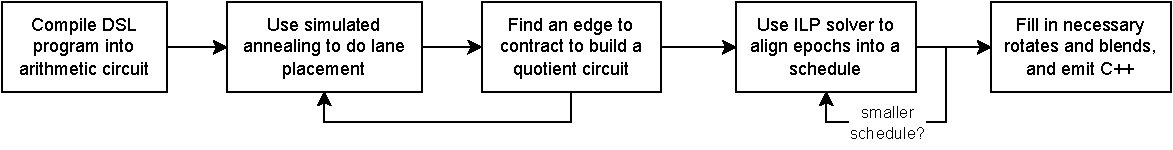
\includegraphics[width=0.8\linewidth]{figures/coyote_algorithm_overview.drawio.pdf}
    \caption{High-level compilation steps}\label{fig:high-level-compilation-steps}
    \Description{Flowchart describing the steps to Coyote's compilation algorithm}
\end{figure*}
\system provides an embedded DSL (eDSL) that allows programmers to use a high level language to express computations in FHE. This computation is translated into an arithmetic circuit representing the computation, which is then compiled into vectorized FHE code. The process of compiling a circuit into vectorized code is as follows: %\milind{overview figure?}

% \milind{You should put the step-by-step procedure for coyote here, then describe them in more detail: break the computation down into aligned subgraphs, assigning scheduling slots, choosing lanes. This is also a good place for a picture explaining these steps: show a tree, show picking bits of a tree, show moving when the computations happen around, show lane assignment}

% \milind{This whole section will benefit from having a running example :-)}
 
\subsection{Compilation Steps}
\begin{figure}
    \begin{subfigure}{0.45\columnwidth}
        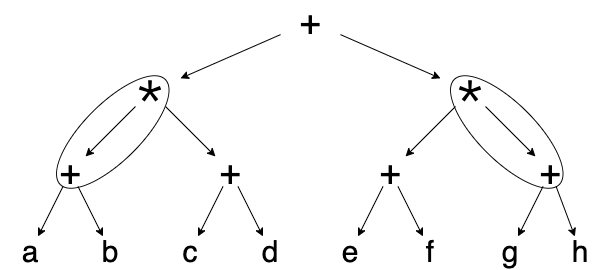
\includegraphics[width=0.9\linewidth]{figures/compilation_overview/running_example_quotiented.drawio.png}
        \caption{Circuit with subcircuits identified}
        \label{fig:subcircuits-identified}
    \end{subfigure}
    \begin{subfigure}{0.45\columnwidth}
        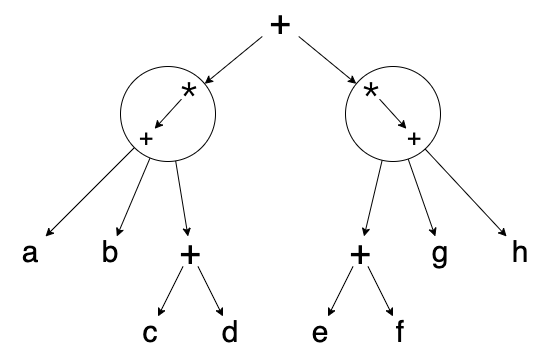
\includegraphics[width=0.9\linewidth]{figures/compilation_overview/running_example_identified.drawio.png}
        \caption{Quotiented circuit}
        \label{fig:quotiented-circuit}
    \end{subfigure}
    \begin{subfigure}{0.55\columnwidth}
        \centering
        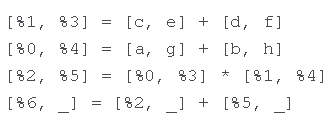
\includegraphics[width=0.9\linewidth]{figures/compilation_overview/aligned_schedule.drawio.pdf}
        \vspace{-1em}
        \caption{Vector schedule after alignment}
        \label{fig:aligned-schedule}
    \end{subfigure}
    \begin{subfigure}{0.4\columnwidth}
        \centering
        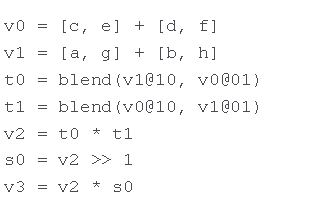
\includegraphics[width=0.9\linewidth]{figures/compilation_overview/generated_vector_ir.drawio.pdf}
        \vspace{-1em}
        \caption{Generated vector code}
        \label{fig:generated-code}
    \end{subfigure}
    \caption{A running example of how \system vectorizes arbitrary arithmetic circuits}
    \label{fig:toy-running-example}
    \Description{Samples of generated code using no vectorization, overly aggressive vectorization, and the optimal vectorization.}
\end{figure}

This section gives an overview of how \system vectorizes an arbitrary arithmetic circuit using the process laid out in Figure~\ref{fig:high-level-compilation-steps}.
We will use the circuit in Figure~\ref{fig:example-circuit} as a running example.
Compilation proceeds as follows:
\begin{enumerate}
    \item \system \textit{quotients} an input circuit (collapses subcircuits into single vertices) and assigns lanes to resulting vertices to produce a {\em pre-schedule} that can be realized into a more efficient vector program. The result is a graph whose vertices correspond to connected subgraphs of the original circuit, such that no two vertices at the same height have the same lane (and hence are eligible to be vectorized together). \system collapses a subcircuit when it determines that the overhead of internally vectorizing it is not worth the gain from vectorization, so this step essentially forces certain operations to happen in scalar on a single lane. %\raghav{I feel I haven't done a good enough job of justifying this.}
    Section~\ref{sec:schedule-search} describes how \system makes this decision. 
    
    In the example in Figure~\ref{fig:subcircuits-identified}, the circled pairs of vertices are collapsed, yielding the quotient circuit in Figure~\ref{fig:quotiented-circuit}.
    The lane assignment for this pre-schedule puts each un-quotiented addition on the same lane as its quotiented parent, and chooses one of these lanes on which to place the root of the tree.
%     \raghav{better?}\milind{This is confusing. Does ``bottom level addition'' mean the addition {\em inside} the subcircuit? Or the other addition that isn't quotiented? I think you need to be more explicit about which operations you're talking about here.} Note that this lane assignment is not intended to be optimal (hence, is a pre-schedule).\raghav{what does this last part mean?}
    
%    \raghav{where do I put this?}
    
    \item The (collapsed) vertices at each height are aligned to pack together isomorphic nodes, producing a vector schedule from the pre-schedule. 
    In the example, the two adds at height 1 get trivially aligned, and the two ``supernodes'' at height 2 get aligned by packing together the two adds and the two multiplies.
    % Since there is a single vertex at height 3, no alignment needs to be done there. 
    No alignment is needed for the single vertex at height 3.
%    \raghav{Is this description clear?}
    The details of the alignment procedure are given in Section~\ref{sec:instruction-alignment}.
    Figure~\ref{fig:aligned-schedule} shows the result of this alignment.
    
    \item \system compiles the schedule into a vector IR. The crux of this compilation step is figuring out when to {\em blend} and {\em rotate}. When a vector operand requires values from several different instructions, \system emits code to ``blend'' the results together into a single vector.
    When the lane an operand is used in is different from the lane it was produced in, \system emits a rotation instruction to move the operand into the correct lane. Notice that each arc in the pre-schedule connecting vertices of different lanes corresponds to a rotation in the generated vector IR.
    Figure~\ref{fig:generated-code} shows the vector code \system generates for our running example.
    Notice that the generated code contains two blends and one rotate.
    The blends are necessary\footnote{In this particular example, exchanging the positions of {\sf \%3} and {\sf \%4} would have produced semantically equivalent code that does not require the blends. However, automatically performing arithmetic rewrites such as this one is outside the scope of this work.} because on line 3 of the schedule, {\sf \%0} and {\sf \%3} are used in the same vector despite being produced in two separate vectors. 
    Since none of the operands need to shift lanes, the vector instruction {\sf t0 = blend(v0@10, v1@01)} takes {\sf [\%0, \%4]} and {\sf [\%1, \%3]} and blends them together to produce {\sf [\%0, \%3]}, which is exactly the operand used on line 3. 
    \system emits a rotation because {\sf \%5} gets used on a different lane than it is produced.
    The vector instruction {\sf s0 = v2 $\gg$ 1} takes {\sf [\%2, \%5]} in {\sf v2} and produces {\sf [\%5, \%2]} in {\sf s0}.
    Section~\ref{sec:codegen} describes the specifics of code generation.
\end{enumerate}
% \raghav{TODO: maybe change the inline texttt stuff so it looks better?}\milind{I tend to prefer {\em {\sf sans serif}} for typesetting inline code, even though it's not monospace}

% \begin{enumerate}
%     \item \system first identifies highly vectorizable subcircuits (shown highlighted in Figure~\ref{fig:small-expr-circuit})
%     \item These subcircuits are pulled out and aligned to produce a single vectorized computation, which is then inserted back into the original program, resulting in the circuit in Figure~\ref{fig:partially-vectorized-circuit}.
%     The challenge with this is aligning the subcircuits optimally; i.e., figuring out which computations can be grouped together into vector operations.
%     Doing this once effectively replaces several subcircuits of the program with a single vectorized circuit, so the process is repeated until no more subcircuits can be found.
%     Each vectorized circuit creates an {\em epoch}, as seen in Figure~\ref{fig:code-split-epochs}.
%     Since the outputs of one epoch are consumed by subsequent epochs, we need to place the outputs in appropriate spots to ensure that the dependences line up.
%     \item The new circuit is converted to a vector {\em schedule} (Figure~\ref{fig:vector-sched-needing-rotates}), which amounts to assigning a {\em lane} (horizontal position) and {\em schedule slot} (vertical position) to each original scalar instruction.
%     \item \system compiles the vector schedule into a vector IR. The crux of this compilation step is figuring out when to {\em blend} and {\em rotate}. When a particular vector operand requires values from several other previously produced vectors, \system emits code to ``blend'' these together into a single vector which can then be used.
    
%     To see why rotates are necessary, notice that in the example schedule, the scalar \texttt{\%3} is computed on lane 2, but used in lane 1. 
%     To correct this discrepancy, \system emits an additional instruction to create a copy of the \texttt{[\%1, \%3]} vector with data arranged as \texttt{[\%3, \%1]}, putting \texttt{\%3} on lane 1 where it is used. %\raghav{Does this flow better?}\milind{yup}
%     % \raghav{Should (3) and (4) go together? Technically (4) is codegen which to me seems like a separate phase of compilation}\milind{It is, but it flows weird -- it's basically a consequence of lane assignment... Or at the very least, write this as a general codegen step, with reference to this example. Right now, it reads as ``this is one specific thing we do'' rather than ``inserting rotation instructions is how codegen works.''}
% \end{enumerate}

% enumerate
% add figure
% \milind{This dives in too quickly; I think the overview thing I laid out above is necessary. Otherwise: what's a stage? What does it mean to schedule subgraphs together? What does it mean to ``line operands up.''}
% \raghav{Is this better? I kind of briefly mentioned ``creating a vector schedule'' as a separate thing that needs to happen apart from just picking vectorizable trees, should I say any more or less about that here, before discussing it in detail in Section~\ref{sec:design}?}
% \system reduces the search space for vectorized programs \raghav{Does it make sense to call it ``search space''?} by first splitting the computation into multiple stages, and only allowing for vector rotations to line operands up between stages.
% A stage consists of a set of independent subgraphs of the entire circuit \raghav{Do I need to explain what independent means here?}. 
% The subgraphs are scheduled together, with each one being placed on its own vector lane. 
% Once vector code for a stage has been generated, all of its subgraphs are removed from the circuit, and the subgraphs for the next stage are picked out.
% After the entire circuit has been split up into stages, the subgraphs from each stage are assigned specific vector lanes to minimize the number of distinct rotations required to line up the outputs of one stage with the inputs of the next.
% Finally, \system computes and inserts these rotation instructions between stages and emits the vector code.

\subsection{Using \system}\label{sec:using-coyote}
\begin{figure}
    \small
    \begin{minted}[linenos,escapeinside=||]{Python}
def dot(v1, v2):
    return sum([a * b for a, b in zip(v1, v2)])|\label{code:zip}|
  
@coyote.define_circuit(A=matrix(3, 3), b=vector(3))
def matvec_multiply(A, b):
    result = []
    for i in range(len(A)):|\label{code:for_loop}|
        result.append(dot(A[i], b))
    return result
    \end{minted}
    \vspace{-1em}
    \caption{\system program for multiplying a vector by a matrix}\label{fig:coyote-program}
    \Description{Example of a program written in \system that implements a matrix/vector multiply}
\end{figure}
A programmer can use {\system}'s DSL (shown in Figure~{\ref{fig:coyote-program}}) to specify a computation and generate an arithmetic circuit. %\milind{move example here}
The DSL exposes a number of ways to annotate inputs to the computation:{\em  replication, }{\em packing}, and fixing a{\em layout}.
Annotating an input with ``replicate'' indicates that a copy of the input should be passed to the circuit for each place it is used (ensuring that each copy gets used exactly once).
By default, inputs are unreplicated, meaning that an input that gets used in multiple places will have a fan-out corresponding to its usage frequency.

Specifying a ``packing'' constraint for a set of inputs requires that they be packed into a single input vector in the final circuit (note that inputs in the same vector are necessarily in different lanes).
For example, a packing constraint might require that each entry of a matrix be placed in the same input vector.

After {\system} vectorizes the circuit as described above, it automatically packs the circuit inputs into vectors (while satisfying any provided packing constraints) and chooses the data layouts within these vectors.
Alternatively, the programmer can choose to override this and manually provide an input layout. %\milind{maybe clarify that the layout choice is for inputs and outputs?} 
This is useful, for example, when composing multiple circuits, as the output layout of one determines the input layout of the next.
The details of how these choices are made are discussed in Section~{\ref{sec:data-layout}}, and the tradeoffs these annotations provide are discussed in Section~{\ref{sec:surface-language}}.
\subsection{Backend}
\system targets the BFV backend \footnote{We could have instead chosen to use the CKKS backend, but BFV's cost model is more amenable to general vectorization. In particular, an operation we use often is ``blending'' slots from several vectors into one; while this is almost free in BFV, the cost of doing this in CKKS is nontrivial. } for Microsoft SEAL\cite{seal}.
The encryption parameters are hardcoded, and are chosen to allow for 8192 vector slots and a standard 128 bits of security.
\section{Design}\label{sec:design}
Naively vectorizing arbitrary arithmetic circuits looks a lot like SLP: we start by serializing the circuit into a sequence of scalar three-address instructions.
At each step, we look at all available scalar instructions (i.e. instructions whose source operands have all already been scheduled), pick the largest set with the same operation, and schedule them together.
The problem with this naive strategy is it makes no guarantees about values being computed and used on the same lane; in other words, it incurs arbitrarily many shuffles to make the computation line up.
Unlike in normal vectorization, where applying arbitrary permutations to the lanes is relatively cheap, in FHE we are only allowed to rotate the entire vector by a fixed number of slots, and this rotation operation is expensive.
Hence, the cost of bookkeeping quickly outweighs whatever benefit we might get from vectorization, making this approach not worth it.

Data movement is actually impossible to avoid: in an arithmetic circuit that computes a single expression, all the intermediate nodes eventually feed into the root\milind{I think we want to consistently talk about these as dependence graphs, where data flows down and things feed into the {\em last} instruction, rather than as expression trees where results flow up and computation resolves at the root...} meaning that without data movement every instruction must be on the same lane; in other words, no vectorization can take place.
Here we have two extremes: on one end of the spectrum is SLP, which packs aggressively without considering data movement; the other end avoids data movement entirely, precluding any vectorization within individual expressions.
The key idea of our approach is to balance between these two extremes, by finding highly vectorizable groups of subexpressions and evaluating those subexpressions together with each one on its own lane.
% don't be specific about trees here
\subsection{Selecting Vectorizable Subexpressions}\label{sec:selecting-subexpressions}
\subsubsection*{Measuring subexpression vectorizability}
We want to measure how well the instruction sequences corresponding to two arbitrary expressions line up.
Given an arithmetic circuit, we can inductively compute the structural similarity between every pair $(t_1, t_2)$ of independent subcircuits (two circuits are independent if they have no overlap) as follows: \milind{Hmmm... I guess here we're pretty tied to the expression tree representation of circuits, so forget what I said earlier about thinking in terms of dependence graphs. Maybe make clear in section 2.1.2 that we'll think of circuits as expression forests or expression DAGs, where leaves are data and interior nodes are operations}

\begin{align*}
    sim(t_1, var) &= 0\\
    sim(var, t_2) &= 0\\
    sim(t_1, t_2) &= \max \begin{cases}
        sim(t_1.L, t_2)\\
        sim(t_1.R, t_2)\\
        sim(t_1, t_2.L)\\
        sim(t_1, t_2.R)\\
        sim(t_1.L, t_2.L) + sim(t_1.R, t_2.R) + b\\
        sim(t_1.L, t_2.R) + sim(t_1.R, t_2.L) + b
    \end{cases}
\end{align*}
where $b = 1$ if $t_1.op = t_2.op$ and $b = 0$ otherwise. \milind{need: explanation of what $L$, $R$, $var$ are, and a plain english intuitive explanation}

For example, in the circuit from Figure~\ref{fig:small-expr-circuit}, we have a similarity score of $2$ between $(ab + c)$ and $(xy + z)$.

% The base case is comparing any tree to a leaf node (a single variable with no operations), in which case the similarity is $0$, as there are no operations that can be packed together.

% In the inductive case of two nontrivial trees, there are six ways they could be lined up: \raghav{TODO: diagram}
% Either root could be lined up with either child of the other tree in four ways. 
% Or, the two roots could line up, giving two ways for their children to line up (left with left and right with right, or left with right and right with left).
% In the first four cases, the similarity score of the two trees is the similarity score of the alignment. 
% In the last two cases, the similarity score of the two trees is the sum of the scores of the aligned children, plus a 1 if the roots have the same operation.
% The final similarity score of the two trees is the maximum possible score out of all six cases. 
% \raghav{This makes no sense even to me, and I was looking at the code when I wrote this.}\milind{Actually, now that I think about it, maybe write this as a set of recurrence relations, a la smith waterman}

\subsubsection*{Choosing maximally vectorizable sets}%\raghav{TODO: add a running example $(ab+c)(xy+z)$}
Not every pair of subexpressions is eligible to be vectorized together, since they have to be independent of each other.
This data can be encoded in an undirected {\em vectorizability graph}, where each subexpression is a vertex, and there is an edge between two vertices if the corresponding subexpressions are independent (and thus vectorizable).
Cliques in this graph correspond exactly to sets of expressions that can all be vectorized together. 
We can further label each edge with the similarity score of the two subexpressions it connects.
Since each similarity score roughly corresponds to the number of instructions that could be packed together, the total weight of a clique represents the total number of operations we save by vectorizing together all the subexpressions contained within. 
There is a subtlety here: we don't just want to take the largest clique in the graph, since this means vectorizing a lot of expressions, which will likely incur several rotates down the line. 
To account for this, we subtract a fixed \milind{Not fixed---based on size of the clique} amount from the weight of each edge; this penalizes large cliques, and ensures that we prioritize finding small cliques of highly vectorizable expressions to avoid doing too many rotations. \milind{Be more vague about this subtraction bit, since we maybe don't do it exactly like that anymore :-) You can add something in implementation that's specifically about the weighting...}
% By simply subtracting a fixed amount from the weight of each edge we can penalize large cliques which would incur a much higher rotation overhead, unless the vectorizability of the clique is high enough to be worth it. \milind{Rephrase this: start by explaining why you don't want to just take super big cliques -- it doesn't take into account rotation -- and then explain how you adjust the weights to account for this}
The problem of finding a set of subexpressions to vectorize together reduces to finding a maximal weight clique in this graph, which is easily packaged off to an SMT solver.

This effectively greedily selects a set of expressions to vectorize, which amounts to scheduling the first {\em epoch} of the program. We want to repeat the process until the entire program has been scheduled.
Repeating the process requires some extra work: whenever a set of subexpressions is selected, each one needs to be ``quotiented out'' of the original program (i.e. collapsed to a new leaf node in the circuit).
Doing so requires that we make two changes to the vectorizability graph:
\begin{enumerate}
    \item All the nodes that were cut out of the circuit (the {\em sub}-subexpressions) need to be eliminated, since they have already been scheduled.
    \item Removing certain subexpressions changes the structure of the larger expressions containing them, and hence changes the similarity of those larger  expressions in the overall circuit. \footnote{This is in contrast to what one might expect when vectorizing at the level of instructions instead of subexpressions. The reason we vectorize at the level of subexpressions is to reduce the total number of epochs, and hence the total number of rotations.} These changes need to be reflected by updating the weights of the vectorizability graph. To handle this more efficiently, we track all the pieces that make up the weight of an edge when computing similarities. These weights can then be updated without having to recompute everything each time. \raghav{How's that?}\milind{works}
\end{enumerate}

Using the circuit from Figure~\ref{fig:small-expr-circuit} as a running example, the maximal weight clique in its vectorizability graph is just the edge connecting $(ab + c)$ and $(xy + z)$ (which from earlier has a weight of 2), so \system selects them to vectorize in the first epoch.
After quotienting them out, the remaining expression is just $(L_1 \times L_2)$ where $L_1$ and $L_2$ correspond to the new leaf nodes the subexpressions get collapsed to.
Since there are no subexpressions here that can be vectorized, \system chooses the whole thing for the second and final epoch.
% A single round of this technique greedily selects the optimal ``breakpoints'' up to which to vectorize before inserting rotations, so we need to iterate until the entire program has been scheduled. \milind{This doesn't make sense to me... I think it'll help to have the overview section already talk about stages, so you can explain this in terms of that.}
% Once a set of breakpoints is selected \raghav{Yeah, this is the first time I'm officially using the word breakpoint so far, I should introduce it earlier. Terminology is {\em hard}.}, they need to be ``quotiented out'' (i.e. each subexpression needs to be replaced by a single leaf node in the expression tree).
% This has two effects on the vectorizability graph: First, all the nodes that appear in the quotient need to be eliminated (including the {\em sub}-subexpressions of the chosen subexpressions), since they are no longer eligible to be vectorized.
% However, removing these subexpressions also affects the similarities of their ancestors, since they now have fewer operations that can be packed together.
% These changes must be reflected by updating the weights of the vectorizability graph.
% To avoid having to recompute all the similarities each time, we store for each edge the list of operations it could pack together; the edge weight can be recovered as the sum of the costs of all of these (in the simplest case, the length). \milind{very confusing...}
% Each time a node is quotiented out, it is removed from each list that contains it; doing so automatically updates all the edge weights to account for its removal.
% \raghav{To deal with point (2) more efficiently, I do a trick where I track all the pieces that make up the weight of an edge, so I can update the weights without having to recompute similarity. I originally tried to write this out, but its kind of confusing. Now that I think about it, though, it seems like more of an implementation detail than anything. Should I still write it out here, or just leave it?}\milind{What you wrote in this comment is sufficient, and it's short enough that it's worth including. It {\em is} sort of an implementation detail, but we can cut it for space if we need to.}
Now, we can repeat the above process of finding a maximal clique and vectorizing it, until eventually all nontrivial cliques have a negative total weight, meaning that there are no more subexpressions that are vectorizable enough to make the rotation costs worth it, so we just emit scalar code for the rest of the program.

\subsection{Instruction Packing}\label{sec:instruction-packing}
Given a set of subexpressions to compute in a single epoch of the program, we can align the instructions between subexpressions to actually produce a vector schedule.
It may seem like the solution to this is just sequence alignment, but aligning circuits is actually more complicated than that.
At each step, the number of available children that can be aligned roughly doubles, meaning that the total number of subproblems to solve is exponential in the depth instead of linear. 
This causes the dynamic programming strategy of sequence alignment to quickly blow up.
% Aligning trees is more complicated than a simple sequence alignment, because at each step the number of available children to align roughly doubles, meaning that the total number of subproblems to solve is exponential in the depth instead of linear. 
% \raghav{Is this a good enough explanation for why sequence alignment doesn't work here?}\milind{Don't just say sequence alignment out of the blue. You want to say something like "It may seem like the way to go is sequence alignment but ..."}

Instead of wrangling so many subproblems, we can formulate this as an ILP.
We create a variable for each scalar instruction representing its {\em schedule slot}, or the time at which it executes.
We add constraints to require that each instruction be scheduled after all of its dependences have been scheduled, and also to require that two instructions with different operations never be scheduled at the same time. 
Finally, to speed up the search for a solution, we place a bound on the total length of the schedule (in other words, an upper bound on the value of the schedule slot for any scalar instruction).
The bound is initially very loose but we iteratively tighten it until the solver returns UNSAT, meaning no smaller schedule could be found, so the most recent one was the smallest.

% Instead of wrangling so many subproblems, we can easily pass this off to an SMT solver. \milind{Maybe say that you formulate this as an ILP? "pass to an SMT solver" is an implementation decision -- the {\em design} is that you create a bunch of ILP constraints}
% The encoding consists of a variable for each instruction representing when it gets scheduled, as well as constraints that require two instructions scheduled at the same time to have the same operation, and constraints that require the two dependencies of each instruction to be scheduled before it.
% Finally, to speed up the search for a solution, we place a bound on the maximum number of slots in the schedule (i.e. the latest time an instruction can be scheduled).
% This bound is initially very loose, but once a schedule is produced we iteratively tighten it until the solver returns UNSAT, meaning no smaller schedule could be found. 
% To prevent compilation from taking too long, we also set a timeout after which the solver simply returns the best available schedule.
% Of course, this means that the vector schedule is no longer guaranteed to be optimal, but this timeout can be adjusted, allowing for a tradeoff between compilation time and optimality.
% sequence of four figures: (a) dependency graph [2 stages] (b) written out list of constraints (c) colored hypergraph (d) colored dependency graph
\subsection{Lane Placement}\label{sec:lane-placement}
% \milind{This subsection definitely needs a couple of figures: Fig 1: here's some expressions, here's what a ``dumb'' lane placement looks like, here's what a ``good'' lane placement looks like. Fig 2: Here's some expressions. Here's the set of constraints we need to use to capture lane placement constraints. Here's the hypergraph that we derive from those constraints. Here's what it looks like when colored. See how it looks like the ``good'' lane placement?} \raghav{``Correspond'' is also becoming an overused word}
\begin{figure*}
    \begin{subfigure}{0.24\textwidth}
        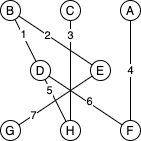
\includegraphics[width=0.9\textwidth]{figures/hypergraph_coloring/small_dependency_graph.drawio.png}
        \caption{A depdendency graph for a simple 3-epoch computation}\label{fig:dependence-graph}
    \end{subfigure}
    \begin{subfigure}{0.24\textwidth}
        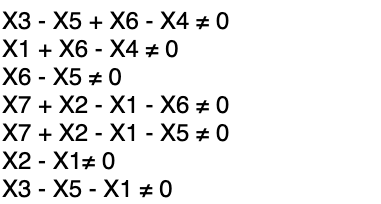
\includegraphics[width=0.9\textwidth]{figures/hypergraph_coloring/hypergraph_relations.drawio.png}
        \caption{The path relations induced by the dependency graph}\label{fig:path-relations}
    \end{subfigure}
    \begin{subfigure}{0.24\textwidth}
        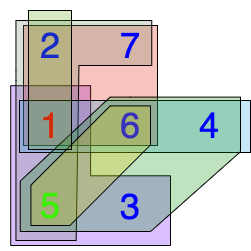
\includegraphics[width=0.9\textwidth]{figures/hypergraph_coloring/colored_dependency_hypergraph.drawio.png}
        \caption{A minimal coloring of the hypergraph corresponding to the path relations}\label{fig:colored-hypergraph}
    \end{subfigure}
    \begin{subfigure}{0.24\textwidth}
        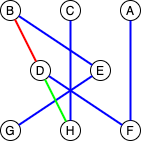
\includegraphics[width=0.9\textwidth]{figures/hypergraph_coloring/colored_dependency_graph.drawio.png}
        \caption{The coloring applied to the original dependency graph. Edges with the same color correspond to the same rotation amount.}\label{fig:colored-dependence-graph}
    \end{subfigure}
    \caption{An example coloring the edges of a dependency graph to produce a good lane assignment}\label{fig:lane-assignment}
    \Description{TODO: insert description}
\end{figure*}

Once the entire program is scheduled, each epoch produces a set of outputs which may feed into inputs of subsequent epochs.
Since no rotation happens within an epoch, each input of an epoch must be on the same lane as the output of the epoch it eventually flows into.
This creates a dependence between the output of one epoch with the output of a downstream epoch, in the sense that if these do not map to the same lane, we need to insert a rotation to line them up.
% Once the entire program is scheduled, each epoch produces a set of outputs which may depend on outputs from previous epochs.
% Each output is produced on a single lane, and whenever a pair of outputs with a dependence between them do not map to the same lane, we need to insert a rotation to get them to line up. \raghav{is this better?}

% Scheduling the program in the way described above amounts to splitting it into a number of {\em epochs}, where each epoch consists of a set of subexpressions to compute. \milind{again ``phase'' vs ``stage''. Also, what's important here isn't that you have the phases -- what's important is that each phase generates output operands in particular lanes, and those operands might need to hook up to one or more input operands in other phases, which means that either the lanes need to be set so everything lines up right, or you need to add rotations.}
For a program that is split into $k$ epochs, we can represent these dependencies in a $k$-partite graph, where each partition corresponds to a epoch and each vertex in a partition corresponds to a subexpression computed in that epoch.
Figure~\ref{fig:dependence-graph} shows an example 3-partite dependence graph for a particular 3-epoch program, where the first epoch had three subexpressions in it, the second had two, and the third had three.
To assign lanes to the subexpressions, we need to assign a number to each vertex in this dependence graph so that no two vertices in the same epoch get the same number.
Unfortunately, a naive approach to this can have very poor results: consider, for example, placing B, D, and G on lane 1; C, E, and F on lane 2; and A and H on the lane 3.
This particular placement requires one rotation each to line up B with E, A with F, and C with H, an additional two rotations to line up D with H and F, and a final rotation to line up E with G.
In the worst case, this incurs 6 rotations.
In the best case, if the vector schedule happens to pack the outputs of B and C together into the same vector, the $B\rightarrow E$ and $C\rightarrow H$ rotations are the same (since they are both a rotation of 1); similarly, if D and E are packed into the same vector, the $D\rightarrow F$ and $E\rightarrow G$ rotations are the same, requiring a total of 4 rotations to line everything up. \raghav{I feel like this is important to say since its the crux of the whole ``use the same number for multiple edges if possible'' thing, but I don't know that I did a good enough job explaining it.}\milind{I think this is good.}
% This particular placement requires one rotation to line B up with E, an additional two rotations to line D up with H and F, respectively, and a final rotation to line up E with G, incurring a total of four rotations. 
But we can do better: if we instead place B, E, and G on lane 1, A, D and F on lane 2, and C and H on lane 3, we can align the epochs with only two rotations: one to line up B and D, and one to line up D and H. 
The goal of the lane assignment algorithm is to automatically determine that optimal placement.

The heuristic approach is to place vertices on lanes while getting as many edges as possible to have the same rotation along them.
It would be much easier to reason about this by assigning rotation values to edges instead of assigning lanes to vertices: a positive value on the edge represents rotating the value to the right before continuing the computation, a negative value represents rotating the value to the left, and a zero represents no rotation.\milind{check}. But note that there is a subtlety we need to keep track of here: not every assignment of rotation values to edges comes from a consistent assignment of lanes to vertices. 

There are two consistency requirements: If the same input value (which is in a particular lane) flows through different operations to the same output value (which is in a particular, possibly different, lane), then all the rotations along the two sequences of operations should eventually place the results on the same lane to generate the output. On the other hand, if the same input value flows to two {\em different} outputs, then the rotations along those two paths {\em must} place the final results in different lanes. \milind{does the preceding explanation of the consistency requirements make sense?} \milind{Maybe give an example of what an inconsistent rotation set looks like.}

This consistency requirement be reworded as follows: for any path that starts and ends on the same epoch in the dependence graph, the {\em directed sum} of the rotation values along it should be zero if the path is a cycle, and nonzero otherwise.
(In a directed sum, we assign a direction to each edge, and negate its value if we follow the edge backwards).
Notice that this automatically enforces that two different paths between a pair of vertices should add up to the same value, since any two such paths also form a cycle by inverting one of them, and the cycle needs to add up to 0. 
% Instead, we try to assign lanes in a way that minimizes the number of {\em distinct} rotations required for each vector (for example, if multiple pieces of data on the same vector are produced two lanes away from where they are consumed, we can rotate the vector a single time to get them both to line up).
% In other words, given a $k$-partite graph with an integer associated to each vertex, we can assign to each edge the difference of its two endpoints, representing the rotation. 
% To minimize the distinct numbers we have to assign to the edges, we'd like to be able to go backwards: in other words, we want to assign as few numbers as possible to all the edges such that ``integrating'' them gives a consistent assignment of numbers to the vertices.

% This consistency constraint can be reworded as follows: For every path through the $k$-partite graph that starts and ends on the same partition, the directed sum of the edge weights along that path must be 0 if the path is a cycle, or nonzero otherwise.
% (Notice that this automatically enforces the condition that two different paths between a pair of vertices on the same partition must add up to the same value, since concatenating one path with the reversal of the other produces a cycle, which must sum to 0).
% \raghav{If only I could figure out a neat and tidy way to describe this whole process mathematically\dots}

Iterating over all the paths in the graph, we end up with a bunch of linear {\em path relations} as shown in Figure~\ref{fig:path-relations}, where initially all of the $X_i$s are unassigned.
To assign a particular $X_i$, if it is part of a relation where it is the only unassigned variable, its value is fixed to be one that satisfies the relation; otherwise, it can be assigned freely.
These constraints form a hypergraph like the one in Figure~\ref{fig:colored-hypergraph}, where the vertices $1,\dots, 7$ correspond to edges in Figure~\ref{fig:dependence-graph}, and each path relation becomes a hyperedge connecting the associated vertices.
In order to find a consistent assignment of rotation values to edges we need to color this hypergraph in such a way that the last vertex to be colored on any hyperedge must be given a distinct color from the rest of the vertices on the hyperedge (this is equivalent to producing a fresh value for the last $X_i$ to be assigned in a path relation, so it can freely be assigned to satisfy the relation). \raghav{Better explanation?}\milind{seems ok}
To minimize the number of distinct rotations needed, we would like to use as few colors as possible.
This is relatively straightforward to do: At each step we pick the vertex that is part of as few ``free'' hyperedges as possible and assign it the next available color, until all the vertices have been colored.
In the example shown in Figure~\ref{fig:colored-hypergraph}, we first assign to $X_3, X_4$, and $X_7$, (hyperdegree 2), then to $X_2$ and $X_6$ (hyperdegree 3), and then to $X_1$ and $X_5$ (hyperdegree 4).
Since $X_1$ is the last vertex to be assigned in the relation $X_2 - X_1 \neq 0$, it must be given a color other than blue, so it gets red, and since $X_5$ is the last to be assigned in the relation $X_3 - X_5 - X_1 \neq 0$, it cannot be red or blue, so it gets green.

Once the vertices of the hypergraph are colored, we can use it to color the edges of the original dependence graph, like in Figure~\ref{fig:colored-dependence-graph}. 
Now, all that remains is getting actual rotation for each color. 
This can be formulated as a simple integer program, with a variable $c_i$ for each color, a variable  $v_j$ for each node in the dependence graph, and a constraint for each edge $(v, v')$ colored $c$ to assert $v - v' == c$.
The way we colored the hypergraph ensures that this integer program is always solvable, and the solution tells us exactly which vector lane each instruction should go on.
\section{Implementation}\label{sec:implementation}

This section discusses the implementation details of \system: how programmers write \system programs, how the code is generated, and several design decisions that allow the system, and the programmer, to trade off optimality for other considerations.

% \subsection{An eDSL and compiler for FHE programs}
% \begin{figure}
%     \begin{lstlisting}[language=Python, escapechar=|]
% def dot(v1, v2):
%     return sum([a * b for a, b in zip(v1, v2)])|\label{code:zip}|
  
% @coyote.define_circuit(A=matrix(3, 3), b=vector(3))
% def matvec_multiply(A, b):
%     result = []
%     for i in range(len(A)):|\label{code:for-loop}|
%         result.append(dot(A[i], b))
%     return result
%     \end{lstlisting}
%     \caption{Sample \system program for multiplying a vector by a matrix}\label{fig:coyote-program}
% \end{figure}

\subsection{An eDSL and compiler for FHE programs}
\begin{figure}
    \begin{minted}[linenos,escapeinside=||]{Python}
def dot(v1, v2):
    return sum([a * b for a, b in zip(v1, v2)])|\label{code:zip}|
  
@coyote.define_circuit(A=matrix(3, 3), b=vector(3))
def matvec_multiply(A, b):
    result = []
    for i in range(len(A)):|\label{code:for_loop}|
        result.append(dot(A[i], b))
    return result
    \end{minted}
    \caption{Sample \system program for multiplying a vector by a matrix}\label{fig:coyote-program}
\end{figure}

% \begin{figure}
%     \begin{lstlisting}[language=Python, escapechar=|]
            
% @coyote.define_circuit(signal=vector(4), kernel=vector(2))
% def convolve(signal, kernel):
%     output = []
%     for offset in range(len(signal) - len(kernel) + 1):
%         output.append(dot(kernel, signal[offset:offset+len(kernel)]))
%     return output
  
% @coyote.define_circuit(A=matrix(3, 3), sig=vector(4), ker=vector(2))
% def composed_kernels(A, sig, ker):
%     b = convolve(sig, ker)|\label{code:call-conv}|
%     return matvec_multiply(A, b)|\label{code:call-matvec}|
%     \end{lstlisting}
    
% \end{figure}

\begin{figure}
    \begin{minted}[escapeinside=||,linenos]{Python}
@coyote.define_circuit(signal=vector(4), kernel=vector(2))
def convolve(signal, kernel):
    output = []
    for offset in range(len(signal) - len(kernel) + 1):
        output.append(dot(kernel, signal[offset:offset+len(kernel)]))
    return output
    
@coyote.define_circuit(A=matrix(3, 3), sig=vector(4), ker=vector(2))
def composed_kernels(A, sig, ker):
    b = convolve(sig, ker) |\label{code:call_conv}| # returns a vector of length 3
    return matvec_multiply(A, b) |\label{code:call_matvec}|
    \end{minted}
    \caption{\system programs are normal python functions that can be composed to build larger kernels}\label{fig:coyote-programs-compose}
\end{figure}

\system consists of an embedded DSL (eDSL) in Python that can be used to write FHE programs.
As the example in Figure~\ref{fig:coyote-program} shows, \system programs are just decorated Python functions.
The decorator registers the function as defining a \system circuit, and allows the programmer to specify the function signature (i.e. the size and shape of each of its inputs).
\system currently supports three input datatypes: {\sf scalar()}, {\sf vector(size)}, and {\sf matrix(rows, cols)}.
Inputs annotated with {\sf scalar()} are always replicated and free to be placed anywhere in the vector schedule; by contrast, {\sf matrix} and {\sf vector} inputs are always packed together and by default unreplicated, although the latter option can be overridden.
For a full discussion of these packing and replication options, see Section~\ref{sec:duplicating-inputs}. \raghav{Should I include these sentences here, or just move them down to Section~\ref{sec:duplicating-inputs}?}

\system internally uses a {\sf CoyoteVar} datatype which represents a symbolic encrypted value, and currently supports addition, subtraction, and multiplication.
To produce a circuit, \system creates a number of these {\sf CoyoteVar} variables (as defined by the signature provided in the decorator) and executes the function with these as parameters.
This method of generating circuits means that any Python construct that does not involve performing unsupported operations on encrypted values\footnote{Unsupported operations include using ciphertexts in branching conditions, loop bounds, or array indices.} can be used as normal in a \system program (for instance, the {\sf zip} and list comprehension in Figure~\ref{fig:coyote-program} on line~\ref{code:zip}).
Notably, \system-decorated functions can include for loops with plaintext induction variables (as on line~\ref{code:for_loop} in Figure~\ref{fig:coyote-program}), and can call other Python functions (including other \system programs, as in Figure~\ref{fig:coyote-programs-compose} on lines~\ref{code:call_conv} and \ref{code:call_matvec}) allowing programmers to write individual kernels and then easily compose them into a larger program.
All loops all fully unrolled and nested function calls are fully inlined before compilation.
The generated circuit is then passed to \system's back end, which vectorizes the computation as described in the previous sections, yielding a sequence of primitive vector operations that can be furter lowered into C++ code targeting Microsoft SEAL's backend for BFV~\cite{seal}.


% \system provides an embedded DSL (eDSL) in Python for expressing FHE programs. \system provides a \texttt{CoyoteVar} datatype which represents a symbolic encrypted value, and supports addition, subtraction, and multiplication. Executing a program that uses \texttt{CoyoteVar}s stages the execution into an arithmetic circuit (e.g., adding together two \texttt{CoyoteVar}s produces a \texttt{CoyoteExpr} that captures an abstract syntax tree representing the addition). 

% Programs written in Python can use {\em non}-{\tt CoyoteVar} variables in conditional statements or as induction variables for loops, and these have the effect of selecting from subcircuits to build (in the case of conditionals) or unrolling a sequence of subcircuits (in the case of loops). Note that FHE limitations mean that {\tt CoyoteVar}s cannot be used in conditionals or as induction variables for loops.

% Once the Python program is executed, the generated arithmetic circuit is passed to \system's back end, which vectorizes the computation as described in the previous sections, yielding a set of vector primitives that can be further lowered into C++ code that targets Microsoft's SEAL backend for BFV~\cite{seal}.



\subsection{Code Generation}\label{sec:codegen}
The output of the algorithm in Section~\ref{sec:design} is a vector schedule (i.e. a lane and schedule slot for each scalar, where the schedule slot determines the order in which instructions get executed).

The available vector instructions and their semantics are as follows:
\raghav{Is this table clear?}
\begin{description}
    \item[Vector Add ($dest = v_1 + v_2$)] $dest[i] = v_1[i] + v_2[i]$
    \item[Vector Multiply ($dest = v_1 * v_2$)] $dest[i] = v_1[i] * v_2[i]$
    \item[Rotate ($dest = v \gg n$)] $dest[i] = v[i - n]$
    \item[Blend ($dest = blend(v_1, \dots, v_n)$)] $dest[i] = v_i[i]$
\end{description}

\raghav{Does the table above make this paragraph redundant?}
This schedule is then compiled into the actual vector IR, which supports vector addition, subtraction, multiplication, and rotation instructions, as well as a constant load instruction and a {\em blend} instruction.
A blend instruction does no data movement, but takes several vectors and ``blends'' them together by choosing specific lanes to take from each one.
In practice, this is implemented as a series of plaintext/ciphertext multiplies (where each ciphertext vector is multiplied by a plaintext ``bitmask'' to hide certain lanes), followed by several ciphertext/ciphertext adds, where each of the masked vectors is added together.


Throughout the compilation, we keep a lookup table that maps a (scalar, lane) pair to the name of the vector register containing it.
In particular, there may be several vector registers that contain a particular scalar, but on separate lanes (this results from a rotation of the original register where the instruction was produced).
(For example, the table might say ``The vector register {\sf s2} has scalar 11 on lane 3'').

At every time step, the schedule compiler finds all scalar instructions scheduled to execute.
For each operand, we use the table to look up the name of the register containing that scalar in the appropriate lane.
If the data for a single vector operand comes from multiple registers, we emit a blend instruction.
Once all the operands have been blended and prepared, we emit the appropriate vector add, subtract, or multiply instruction.
We then look ahead to see if any of the scalars produced by this vector instruction get used on different lanes; for each distinct rotation this induces, we emit a vector rotate instruction.
To standardize, all rotation amounts are positive modulo the vector width.
Finally, for each vector register just produced (including the original one and any rotated ones), we add all of its scalars and their lanes to the lookup table and proceed to the next time step.

Once the circuit is compiled to the vector IR, it can be further lowered to C++ SEAL code.
This is a straightforward process, and essentially consists of transliterating the IR. 
SEAL does not support a built-in blend instruction, though, so each of these generate several ciphertext/plaintext multiplies followed by a single ciphertext add.
While lowering to C++, we also precompute all the blending masks, so that we can encode all of them into the plaintext space once at the beginning of the program and just look up the appropriate one to use each time.

\subsection{Optimality Tradeoffs}\label{sec:optimality-tradeoffs} \raghav{Is this the right name for the section?}
Because the instruction alignment phase only happens once a pre-schedule has been computed, the results of alignment are not available to our cost model.
This is by design, since the instruction alignment problem is formulated as an ILP (Section~\ref{sec:instruction-alignment}), and making multiple expensive calls to an ILP solver in each round of the pre-schedule search would quickly make the entire search procedure intractable.
However, this does bear an impact on the cost model, as without alignment results, we are forced to work at the level of granularity of entire epochs, resulting in approximations of the schedule height and number of rotation rotations.

In particular, the approximations tend to underestimate the true cost of the final realized schedule in two ways:
\begin{itemize}
    \item Undercounting the number of rotations
    \item Underestimating the height of a given epoch
\end{itemize}

When counting rotations, we assume that if two cross-lane arcs originate from the same epoch and have the same span, they can be realized with a single rotation instrution.
This assumption fails if the instructions each arc rotates \raghav{(?)} do not get aligned in the final schedule, since there are now multiple vectors in that epoch that require the same rotation.
This is impossible to avoid without fully aligning everything before computing rotation costs, which as mentioned before is intractable; in practice, however, the estimated rotation costs do not differ from the actual rotation costs by too much, so we still get good schedules. \raghav{stronger way to say this? technically the only evidence I have to back this up is ``I looked at the debug output telling me the estimated costs and compared it by hand to the actual cost by counting ops for a couple small benchmarks and didn't see much of a difference''}

The other approximation we make is when computing the ``height'' of a single epoch, we do not take into account dependences between instructions before counting them. 
In other words, if two columns in the epoch each have an add and a multiply, but the add depends on the multiply in one and vice-versa in the other, the alignment would pack together the multiplies and not the adds, resulting in an actual height of two adds and one multiply; by contrast, \system records the height as one add and one multiply.
We could do a more sophisticated analysis at this step to get estimates that are closer to the true height; however, as before, such analyses are often too expensive to do in the inner loop of a search procedure, and in practice, our estimated heights are still sufficient to guide the search towards more efficient schedules. \raghav{same as before, is there a better way to say this without committing to doing a full case study of the differences between estimated and actual costs?}


% Because each of the compilation steps quickly blows up when given larger programs, we make a number of tradeoffs that sacrifice optimality in exchange for faster compilation times.

% \subsubsection*{Finding maximal cliques/synthesizing alignment}\label{sec:iterative-synthesis}
% In many cases, we want a certain optimal solution to the problem we are passing to the solver; for instance, we want the clique with the largest sum of edge weights, or we want the vector schedule that uses the fewest schedule slots.
% One way to accomplish this is to pass an objective function to the solver; however, this technique often takes a long time, since before returning a solution the solver must first prove that no better one exists.
% Instead of supplying an objective function, we first find any legal solution (e.g. any clique, or any schedule that respects instructions and dependences).
% We then add a constraint that require the next solution to be strictly better than the first one, and query the solver again, until eventually it returns ``unsatisfiable'', meaning that no better solution to be found.
% We can then set a time limit so that if no better solution is found within it, we use the best one we have so far.
% By varying the time limit, we can trade off between optimality and compilation time.

% \subsubsection*{Computing graph paths}\label{sec:computing-graph-paths}
% To build the hypergraph described in Section~\ref{sec:lane-placement}, we first need to compute all paths through the dependence graph.
% We start with all paths of length one (edges) and inductively computing transitive closures, keeping track of all the cycles we find along the way.
% For very large or complicated dependence graphs, this can take a very long time, so we once again set a time limit after which we stop looking for paths (in practice, this amounts to choosing a maximum length of path to look for).
% This timeout can result in missing some relations: even a properly colored hypergraph may produce an unsolvable integer program.
% In these cases, the solver produces an ``unsat core,'' witnessing the unsatisfiability as a set of paths through the dependence graph that start and end on the same epoch, but sum to the wrong thing (e.g., a cycle that sums to a nonzero value).
% When we encounter this scenario, we ``uncolor'' all the edges along such paths, allowing the solver to assign them whatever values it needs to in order to make the program satisfiable.
% Doing so breaks certain symmetries (e.g., an uncolored edges may no longer have the same value as another edge, necessitating an extra rotation), but the lane assignment is still correct.
% Once again, this amounts to sacrificing optimality for compilation time: by increasing the time limit on finding the paths, we can avoid missing relations, and ensure that we never have to do this.

\subsection{Input Layout}\label{sec:duplicating-inputs}
The arithmetic circuits input to \system are DAGs, which fail to be trees exactly when values are used as inputs to multiple computations (for instance, in the expression $ab + ac$, the value $a$ is used as an input to both multiplies).
Any such DAG can be turned into a tree, however, simply by creating copies of each repeated value, in a ``reverse-CSE'' process.
%Applying this to the example expression yields $a_1b + a_2c$ where $a_1$ and $a_2$ are fresh input variables that both have the same value passed into them.
By duplicating the data, the new circuit, while strictly bigger, may have better rotation characteristics.
This is because if $a$ were to be used on two different lanes it would have incurred at least one rotation, but by having two copies of $a$ we can avoid this rotation entirely. The frontend DSL for \system exposes an API by which the programmer can specify which of the input variables to the computation should be duplicated, and which ones should not.

Another input layout control the \system DSL exposes is the {\em input grouping} API, which allows a programmer to specify sets of inputs which are forced to be packed together into a single vector.
This is useful, for example, when doing a matrix computation.
By default, \system treats the 9 elements of a $3 \times 3$ matrix as independent inputs to the computation.
However, by putting all of them into the same input group, the programmer can prevent the matrix from having to be split across multiple ciphertext vectors when input to the computation, and generate vector code that operates on a single packed matrix. 
There is a tradeoff: \system may have been able to find a schedule with fewer rotates with two matrix entries on the same lane, but forcing the entire matrix to packed into a single vector precludes any such schedule.

Both of these input controls allow programmers to trade off between predictable input layouts, that are good for composing kernels without too much rotation, and flexible input layouts, that can give \system more flexibility to manage data flow. Rather than automatically trying to balance these factors, \system leaves it up to the programmer.



% \subsection{Weighting Cliques for Epoch Selection}\label{sec:penalizing-rotates}%\raghav{Name this section something different?}
% When choosing cliques to form epochs as discussed in Section~\ref{sec:selecting-subexpressions}, we have the option to penalize the rotation overhead of choosing large cliques by subtracting a fixed amount from the weight of each edge (since a larger clique has more edges, it incurs a higher penalty).
% However, doing so often grossly overestimates the rotation overhead, particularly in highly regular programs, where many of the rotations are mostly independent and can easily be folded into a single rotate instruction.
% This overestimation can lead to picking conservatively small cliques that don't have as much vectorizability, even though a larger clique would have been more vectorizable without incurring too many rotations.
% To detect this, we find two sets of epochs: one with rotation penalties applied to the vectorizability graph, and one with no penalties.
% Compilation proceeds as normal, creating two dependence graphs and then two hypergraphs, and coloring them both.
% At this point, by inspecting the two colorings, we can determine how much worse the rotations are in the non-penalized case, and compare this to the increased vectorizability from using larger cliques.
% The better of the two options is then used for the rest of compilation.

% This does add the overhead of longer compile times, since now the clique finding and hypergraph coloring needs to happen twice instead of just once; fortunately, most of the heavy lifting occurs while determining instruction packing and actual lane placement, both of which only happen once.
%\raghav{Should I add a sentence like ``Furthermore, since you should only be compiling once and then running a bunch of times, we think this is justified''?}\milind{Nah, that's implied, and we can always say it in a rebuttal if we need to.}
\section{Evaluation}\label{sec:eval}

%  \milind{Putting this comment back :-) Need to intro evaluation here: 
%  1. what research questions we're trying to answer, and why. Each RQ (or two) is going to correspond to a subsection of the evaluation.
%  2. high level overview of what we're going to evaluate to answer those questions
%  3. what platforms we're using to do the evaluation
%  }

In this evaluation, we aim to answer the following questions:

%\raghav{flipped the first two around so its in order :)}
\begin{enumerate}
    \item {\bf How effective is \system's vectorization?} To answer this, we count the number of instructions generated in the vector code compared to the scalar code. (Section~\ref{sec:compilation-stuff})
    \item {\bf How much speedup does compiling with \system get us?} To address this, we compile several realistic benchmarks and measure the speedup of the vectorized code over scalar execution. (Section~\ref{sec:speedups})
    \item {\bf \hl{How well does {\system} scale up to larger kernel sizes?}} \hl{To measure this, we compile a much larger circuit by vectorizing and composing its components. (Section~{\ref{sec:scalability}})} %\raghav{does this sound okay}
    \item {\bf How well do \system's schedules compare to hand-optimized code?} We compare the run times of various hand-optimized benchmarks to the run time of the vector code that \system generates for them. (Section~\ref{sec:expert-comparison})
    \item {\bf To what extent does the data layout chosen by the programmer affect \system's ability to vectorize?} We conduct a case study exploring various data layout schemes for a $3\times 3$ matrix multiply, and measure the vectorization speedup for each layout. (Section~\ref{sec:effects-of-data-layout})
   \item {\bf \hl{How effective is the layout/schedule co-optimization strategy?}} \hl{We track the progress of the schedule-search procedure over time for various levels of data layout optimization. (Section~{\ref{sec:search-and-cooptimization}})}
   \item {\bf \hl{How much optimality do we sacrifice by setting synthesis timeouts?}} \hl{We turn off the synthesis timeouts to guarantee optimal schedule alignments and compare the results. (Section~{\ref{sec:ilp-ablation}})}
\end{enumerate}

\subsection{Computational Kernels}

%\raghav{spot-check my tenses?}
To assess \system's ability to vectorize general applications, we use a suite of benchmarks that represent a spectrum of both regular and irregular computations, as well as ones that are both sparse and dense in terms of data reuse.
While there is not currently a standard benchmark suite on which to evaluate FHE-based compilers, we choose a set of benchmarks similar\footnote{While we do not have access to Porcupine's actual benchmarks for a direct comparison, their polynomial regression corresponds to our matrix multiply, their L2 distance correpsonds to our point cloud distance, and most of their image processing kernels are specific convolutions (i.e. plaintext kernels), while we evaluate on generic convolutions. The input sizes of our benchmarks are comparable to those of Porcupine's.} to those used by Porcupine~\cite{Porcupine}, representing a spectrum of both regular and irregular computations, as well as ones that are both sparse and dense in terms of data reuse.

%\raghav{I'm hesitant to say sparse because that means something different}. \milind{Give a couple of sentence description of each, and also say whether we're classifying this as regular/irregular or dense/sparse, and why. Then you can just move the extra stuff about decision tree into the list, too}

The benchmarks are as follows:
%\raghav{I think the wording could be fixed here but I'm not sure how.}
\begin{enumerate}[label=\arabic*.]
    \item Multiplying two matrices. We do this with $2\times 2$ matrices (regular, little data reuse) and $3\times 3$ matrices (regular, some substantial data reuse). %Matrix multiply ($2\times 2$ and $3\times 3$): the $3\times 3$ matrix multiply is somewhat data-dense, since each input is used three times.
    \item Vector dot product, with vector sizes of 3, 6, and 10 (all of these are regular with no data reuse).
    \item 1D convolution. We do this with a vector of size 4 and a kernel of size 2, and with a vector of size 5 and a kernel of size 3. Both of these are regular and have little data reuse.
    \item Point cloud distances (Given a set of points, compute the square of every pairwise Euclidean distance). We do this for 3, 4, and 5 points. These are all regular but have some substantial data reuse, especially in the 5-point case.
    \item Sorting a list of size 3. This benchmark implements the sort as a ``decision tree'', taking as input three ciphertexts representing pairwise comparison results and six ciphertext ``labels'' representing possible arrangements of the sorted list. In particular, each of the three comparison results gets used in multiple branches of the tree. ``grouped'' here means the data layout groups the three comparisons into one vector and the six labels into another. This is irregular, and the grouped versions have data reuse.
    \item \hl{Finding the maximum element in a list of size 5. This benchmark takes as input five ciphertexts representing the elements of the list, and ten ciphertexts representing pairwise comparison results. Similar to the sorting benchmark, this is irregular, and the grouped versions have data reuse.}
\end{enumerate}

%\raghav{redundant?}
%(Notice that the decision tree benchmark contains irregular computation, and the packed decision tree, all the point cloud distances, and the $3\times 3$ matrix multiply are relatively dense in terms of data reuse).

To investigate the effect of data replication we used three different replication strategies for each benchmark: 

\begin{enumerate}[label=(\roman*)]
\item {\em unreplicated}, where each input appears in only one input vector, and hence must be used by multiple operations.
\item {\em partially replicated} in which one of the two inputs is fully replicated---and hence each operation that requires that input gets its own copy, obviating the need for data movement---while the other is not.
\item {\em fully replicated} in which both inputs are fully replicated. 
\end{enumerate}
Note that for dot product, replication makes no difference as each input is used exactly once.

\subsection{Costs and Effects of Vector Compilation}\label{sec:compilation-stuff}

\begin{table*}
	\small
	\centering
    \caption{Compilation time in seconds, as well as instruction counts in the scalar (SAdd, SSub, SMul) and vector (VAdd, VSub, VMul, Rot, Blend) code, and the ideal speedup (work/span). Note that ideal speedup considers rotates and blends to be free.}\label{tab:big-ass}
    \vspace{-0.5em}
    \begin{tabular}{lcccccccc}
    \toprule
    Benchmark & Time (s) & SAdd + SSub & SMul & VAdd + VSub & VMul & Rot & Blend & Ideal Speedup\\\midrule
    conv.4.2.un & 97 & 3 & 6 & 2 & 1 & 4 & 4 & 5.73\\
    conv.4.2.partially & 80 & 3 & 6 & 2 & 1 & 2 & 1 & 5.73\\
    conv.4.2.fully & 71 & 3 & 6 & 2 & 1 & 1 & 2 & 5.73\\
    \midrule
    conv.5.3.un & 206 & 6 & 9 & 3 & 1 & 7 & 5 & 8.0\\
    conv.5.3.partially & 211 & 6 & 9 & 4 & 1 & 4 & 3 & 8.0\\
    conv.5.3.fully & 208 & 6 & 9 & 4 & 1 & 2 & 3 & 8.0\\
    \midrule
    dist.3.un & 228 & 18 & 9 & 1 & 1 & 4 & 6 & 9.82\\
    dist.3.partially & 233 & 18 & 9 & 1 & 1 & 4 & 6 & 9.82\\
    dist.3.fully & 226 & 18 & 9 & 2 & 2 & 2 & 7 & 9.82\\
    \midrule
    dist.4.un & 425 & 32 & 16 & 2 & 2 & 6 & 8 & 17.45\\
    dist.4.partially & 432 & 32 & 16 & 2 & 2 & 6 & 8 & 17.45\\
    dist.4.fully & 463 & 32 & 16 & 2 & 2 & 4 & 8 & 17.45\\
    \midrule
    dist.5.un & 619 & 50 & 25 & 2 & 2 & 13 & 10 & 27.27\\
    dist.5.partially & 629 & 50 & 25 & 2 & 2 & 13 & 10 & 27.27\\
    dist.5.fully & 609 & 50 & 25 & 2 & 2 & 9 & 10 & 27.27\\
    \midrule
    dot.3.un & 10 & 2 & 3 & 3 & 1 & 2 & 0 & 2.67\\
    dot.3.partially & 10 & 2 & 3 & 3 & 1 & 2 & 0 & 2.67\\
    dot.3.fully & 10 & 2 & 3 & 3 & 1 & 2 & 0 & 2.67\\
    \midrule
    dot.6.un & 159 & 5 & 6 & 4 & 1 & 3 & 2 & 5.0\\
    dot.6.partially & 154 & 5 & 6 & 4 & 1 & 3 & 2 & 5.0\\
    dot.6.fully & 156 & 5 & 6 & 4 & 1 & 3 & 2 & 5.0\\
    \midrule
    dot.10.un & 254 & 9 & 10 & 6 & 1 & 5 & 4 & 7.79\\
    dot.10.partially & 257 & 9 & 10 & 6 & 1 & 5 & 4 & 7.79\\
    dot.10.fully & 251 & 9 & 10 & 6 & 1 & 5 & 4 & 7.79\\
    \midrule
    mm.2.un & 176 & 4 & 8 & 2 & 1 & 3 & 2 & 7.64\\
    mm.2.partially & 171 & 4 & 8 & 2 & 1 & 2 & 1 & 7.64\\
    mm.2.fully & 170 & 4 & 8 & 2 & 1 & 1 & 2 & 7.64\\
    \midrule
    mm.3.un & 573 & 18 & 27 & 5 & 2 & 20 & 10 & 24.0\\
    mm.3.partially & 610 & 18 & 27 & 4 & 1 & 18 & 6 & 24.0\\
    mm.3.fully & 607 & 18 & 27 & 4 & 2 & 9 & 3 & 24.0\\
    \midrule
    sort[3].grouped.un & 238 & 10 & 10 & 8 & 4 & 8 & 6 & 3.24\\
    sort[3].grouped.partially & 233 & 10 & 10 & 8 & 4 & 4 & 3 & 3.24\\
    sort[3].grouped.fully & 231 & 10 & 10 & 8 & 4 & 4 & 3 & 3.24\\
    sort[3] & 139 & 10 & 10 & 11 & 5 & 1 & 1 & 3.24\\
    \midrule
    \hl{max[5].grouped.un} & \hl{880} & \hl{30} & \hl{30} & \hl{15} & \hl{11} & \hl{30} & \hl{18} & \hl{7.33}\\
    \hl{max[5].grouped.partially} & \hl{905} & \hl{30} & \hl{30} & \hl{12} & \hl{9} & \hl{27} & \hl{15} & \hl{7.33}\\
    \hl{max[5].grouped.fully} & \hl{902} & \hl{30} & \hl{30} & \hl{19} & \hl{9} & \hl{24} & \hl{23} & \hl{7.33}\\
    \hl{max[5]} & \hl{537} & \hl{30} & \hl{30} & \hl{17} & \hl{6} & \hl{15} & \hl{13} & \hl{7.33}\\
    \midrule
    \hl{mm.16.blocked} & \hl{7139} & \hl{3840} & \hl{4096} & \hl{414} & \hl{128} & \hl{4446} & \hl{872} & \hl{3200}\\
    \bottomrule
    \end{tabular}
\end{table*}


Table~\ref{tab:big-ass} shows benchmark properties, including how long each benchmark took to compile and how many operations each program had before and after vectorization.
Our benchmarks ranged in size from 5 scalar instructions (size 3 dot product) to 75 instructions (5 point distances) %\footnote{Note that \system is able to handle benchmark sizes much larger than those of Porcupine \cite{Porcupine} while maintaining reasonable compile times}.
While the number of scalar multiplies went as high as 27 (for the $3\times 3$ matrix multiply), \system was almost always able to pack these into at most one or two vector instructions.
The main exceptions to this rule were the highly irregular tree benchmarks, which still went from 10 scalar multiplies to between 4 and 5 vector multiplies.
Another point to notice is the number of rotates. Most benchmarks required fewer than 10 rotates. However, the 5 point distance and $3\times 3$ matrix multiply benchmarks had a very high number of rotations after vectorization, as these were the most data-dense ones---intermediate results were required by many downstream computations, incurring considerable overhead. %requiring many rotates.
Furthermore, the unreplicated versions of each benchmark almost always incurred more rotates than the partially or fully replicated versions, validating our hypothesis that input replication helps alleviate the rotation burden. % when vectorizing.
%\raghav{anything else interesting to mention?}

Table~\ref{tab:big-ass} also shows the ideal speedup for each benchmark, using our cost model of multiplies being 10$\times$ as expensive as adds and subtracts. Note that this modeled speedup is based on a classic work/span analysis, and hence assumes that permuting and shuffling data between vectors is free. This modeled speedup thus represents a substantial overestimate of the actual speedup that could be achieved in the program. For example, a \textsf{3x3} matrix multiply has nine 3-element dot products. The necessary 27 multiplies can all be performed in one vector operation, but the results of three multiplies need to be added to perform each dot product (which requires two adds each). Thus in reality two of the multiplies are performed in the ``wrong'' lane and need to be shuffled to the correct lane to complete the computation.
% \milind{There should be a paragraph or subsubsection here that discusses the benchmark table: how big each benchmark is, what the effects of vectorizing it are in terms of operations saved, etc. This is a precursor to discussing anything runtime related.}

\subsection{Speedups}\label{sec:speedups}

\begin{figure}[t]
	\centering
    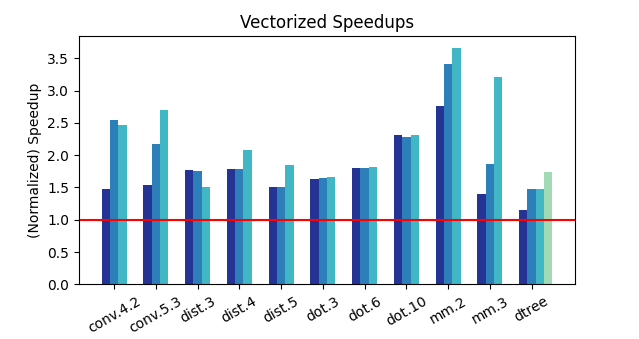
\includegraphics[width=0.9\linewidth]{figures/graphs/vector_speedups.png}
    \caption{Speedup of vectorized code over scalar (higher is better). Left-to-right, the first three bars for each benchmark represent unreplicated, partially replicated, and fully replicated inputs, respectively. The fourth bar for the {\tt sort[3]} and {\tt max[5]} benchmarks represent ungrouped inputs.}\label{fig:vector-speedups}
    \Description{Bar graph showing speedup from vectorization for each benchmark}
\end{figure}

% \milind{This is the punchline to your main research question: ``Can we get vectorization speedup.'' So it should be its own subsection.}
While instruction counts indicate that \system is able to effectively find vector operations for each benchmark, we must also determine whether the actual costs of rotations and blends outweigh the vectorization benefits. Hence, we run each benchmark 50 times in scalar, and 50 times after vectorization to compute the speedup from vectorization, shown in Figure~\ref{fig:vector-speedups}.
%The average speedup is computed as the total scalar execution time divided by the total vector execution time.
We find very little variance in execution time across individual runs for any benchmark.
Each benchmark has three bars representing, in order from left to right, the unreplicated, partially replicated, and fully replicated runs. 
The decision tree benchmark has an extra green bar representing the ungrouped run (without grouping, all inputs are fully replicated no matter what).
We see speedups ranging from anywhere between $1.5\times$ on the data-dense point cloud distances benchmarks to over $3.5\times$ on the highly vectorizable matrix multiply.
We also generally notice more speedup as the replication level increases, suggesting that \system is able to take advantage of replicated inputs to eliminate rotations from the schedule.

While it may appear that \system's actual speedups are sometimes well off from the idealized speedups, this is due to the rotations and blends required to implement these benchmarks outside an idealized world where vector permutation is free. For example, in the \textsf{3x3}, fully-replicated matrix multiply case, \system generates 9 rotations to move results into place. We see, though, that in benchmarks where \system can generate schedules with few rotates, it does well despite the data movement costs. For example, in \textsf{conv.4.2}, \system achieves a 2.5$\times$ speedup versus an ideal speedup of 5$\times$; and in \textsf{dot.3}, \system achieves a 1.6$\times$ speedup versus an ideal speedup of 2.7$\times$.

%\milind{This would be a good place to discuss the comparison of our speedups with rotation vs. modeled ideal speedups without rotation costs...}
\subsection{Scalability}\label{sec:scalability}
\hl{Many of the benchmarks we evaluate on have relatively small input sizes, since it is often intractable to directly apply the search procedure {\system} uses for lane placement.
However, it is possible to scale {\system} up to larger input sizes by ``blocking'', or vectorizing smaller kernels separately and then composing the vector programs.
To investigate how well this scaling works, we used {\system} to compile a $16\times 16$ matrix multiply as follows.
We vectorized the multiplication of a single $4\times 4$ ``block'', and recorded the input/output layouts {\system} chose.

The output layout of each $4\times 4$ block was used to fix the input layout to another kernel (see Section~{\ref{sec:using-coyote}}), which took 64 of these blocks and performed the necessary reductions to arrange them into the final result of the $16\times 16$ matrix multiplication.
The metadata for this benchmark is shown under {{\tt mm.16}} in Table~{\ref{tab:big-ass}} (the compilation time includes the time to compile the $4\times 4$ block as well as the reduction circuit).
After vectorizing, the blocked $16\times 16$ matrix multiply takes 3433 seconds, compared to 4541 seconds before vectorizing, for a total 32\% speedup.
This shows that by composing smaller kernels, {\system} is able to scale up to vectorizing much larger circuits and still see relatively significant speedups over unvectorized code. Note that this understates Coyote's potential speedup as it does not currently attempt to vectorize separate, identical kernels together (which, note, is a regular process so could use standard vectorization techniques).}

\subsection{Randomly Generated Irregular Kernels}
\begin{figure}[t]
	\centering
    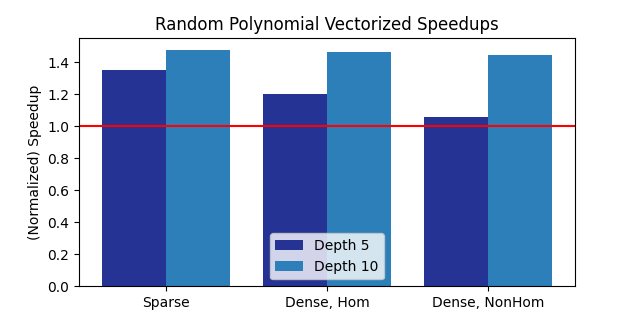
\includegraphics[width=0.9\linewidth]{figures/graphs/trees.png}
    \caption{Speedups for random polynomials (higher is better).}\label{fig:polynomial-speedups}
    \Description{Bar graph showing speedup from vectorization for randomly generated polynomials}
\end{figure}

%\raghav{How can this be said better?}
To further investigate \system's ability to vectorize, even in the absence of a regular structure on the computation, we randomly generated several polynomials to evaluate as arbitrary arithmetic expression trees.
The trees are generated according to three different regimes to cover different kinds of programs: 
\begin{enumerate}
    \item {\em Dense, homogeneous}: The expression tree is both full and complete, and all the operations are isomorphic. In principle, this represents a best case for vectorization.
    \item {\em Dense, nonhomogeneous}: The expression tree is both full and complete, each operation has a 50/50 chance of being an add or a multiply. Hence, while the trees are structurally similar, the heterogeneity of operations means that vectorization opportunities are restricted.
	\item {\em Sparse}: Many operations have one leaf node input, the tree is not very balanced. In principle, this represents a worst case for vectorization, where \system must work hard to find vectorizable computation.
\end{enumerate}
For each regime, we generate ten total polynomials, five with a circuit depth of 5 and five with a circuit depth of 10.
Each polynomial is run 20 times in scalar and 20 times after vectorization, and we average speedups across the five polynomials in each regime before reporting.
These speedups are shown in Figure~\ref{fig:polynomial-speedups}.
We see that \system is able to achieve speedups of up to $1.4\times$ by vectorizing.
Looking at the depth 5 dense nonhomogeneous polynomials, we found that many of them were too small and irregular to admit any profitable vectorization; in these cases, \system was correctly able to deduce that the scalar execution strategy was optimal rather than attempting to vectorize and incur spurious rotations.
Since the generated vector code was identical to the scalar code for several of these, the average speedup is very close to $1.0$.

We find that both sparse and dense homogeneous polynomials see substantial benefits from vectorization, with sparse polynomials having more speedup. This may seem surprising: dense homogeneous trees appear to be a best case scenario for vectorization, as all of the operations can be perfectly packed together. However, the key to this result is that rotations are expensive. The sparse trees have many vertices of arity 1---these operations do not require any rotations to align their input operands. In contrast, the dense trees require more rotations, canceling out the benefits from greater vectorization. This is further justification for \system's design decision to focus on minimizing rotation in its schedule search. In the light of this discussion, it is perhaps {\em un}surprising that the dense trees (requiring more rotation) with non-homogeneous operations (limiting vector packing) ultimately have the lowest speedup.

\subsection{Comparison to Hand-Optimized Schedules}\label{sec:expert-comparison}
To compare \system's vectorized schedules to hand-optimized baselines, we compiled three kernels with \system: matrix/vector multiply, dot product, and point-cloud distance.
Each of these kernels has a well-known expert-optimized baseline implementation, which we also implemented in \system's vector IR, before compiling both to C++ and measuring the time it took to run each one 50 times.
The results are shown in Table~\ref{tab:expert-comparison-numbers}.
For smaller sizes, we see \system's vectorization was capable of matching or even outperforming the expert-written baselines, although on larger sizes the search space was often too big to automatically find the expert schedules.
Manually inspecting the generated code shows that this was usually because the schedule \system generated used one or two more rotates than the baseline.
In the case of the dot product, the schedules \system found all used the same number of rotates as the expert schedule, but occasionally incurred more blends.

\begin{table}
	\centering
    \small
    \caption{\system vectorization vs. expert-written code}\label{tab:expert-comparison-numbers}
    \begin{tabular}{lcc}
        \toprule
        Benchmark & \system time (s) & Expert time (s)\\\midrule
        mv.2 & 2.37 & 2.51 \\
        mv.3 & 3.3 & 3.9 \\
        mv.4 & 7.7 & 5.3 \\
        dist.3 & 3.5 & 3.2 \\
        dist.4 & 8.4 & 4.0 \\
        dist.5 & 15.3 & 5.5 \\
        dot.3 & 1.6 & 1.6 \\
        dot.6 & 2.9 & 2.2 \\
        dot.10 & 3.8 & 2.6 \\
        \bottomrule
    \end{tabular}
\end{table}

\subsection{Effects of Data Layout}\label{sec:effects-of-data-layout}
% \milind{Call this ``effects of data layout.'' There should be a research question in the evaluation intro that directly pertains to this case study.}
To study the effects of different data layout choices, we vary the data layout in $3\times 3$ matrix multiply:
\begin{description}
    \item[Together:] The matrices $A$ and $B$ are grouped into a single vector of $18$ elements
    \item[Separate:] $A$ and $B$ are grouped into individual vectors (this is the normal layout used in benchmarking in Figure~\ref{fig:vector-speedups})
    \item[Rows/Cols:] The rows of $A$ are grouped into three separate vectors, as are the columns of $B$.
    \item[Cols/Rows:] The columns of $A$ are grouped into three separate vectors, as are the rows of $B$.
    \item[Individual:] Each of the 18 entries are grouped into their own vector (note that this is different from simply leaving them as free scalars, because this precludes \system from choosing to put some of them on the same vector anyway).     
\end{description}
%\begin{table}
%	\centering
%    \small
%    \caption{Compilation time and vector operation counts for different layouts of $3 \times 3$ matrix muliply.} \label{tab:bigass-data-layout}
%    % \vspace{-1em}
%    \begin{tabular}{lccccc}
%    \toprule
%    Benchmark & Time (s) & VAdd+VSub & VMul & Rot & Blend\\\midrule
%    together & 584     & 5         & 2    & 15  & 10\\
%    separate & 594     & 5         & 2    & 20  & 10\\
%    rowscols & 565     & 11        & 6    & 24  & 22\\
%    colsrows & 601     & 5         & 3    & 24  & 10\\
%    indiv & 522     & 16        & 13   & 33  & 25\\\bottomrule
%    \end{tabular}
%\end{table}
In each layout, all the inputs are unreplicated.
Figure~\ref{fig:data-layout-case-study} shows the results of this case study.
Interestingly, we find that grouping the matrices together yields greater speedups than keeping them separate.
When multiple entries are on one vector, \system can arrange the elements such that rotating one automatically gives useful rotations of the others.
By contrast, when each entry is on a separate vector, every rotation must necessarily be done separately, so that schedule ends up with much more overhead. In particular, we find that {\tt indiv} requires more than twice as many rotations as {\tt together}.
%This effect can be seen in Table~\ref{tab:bigass-data-layout}: {\tt indiv} incurs over twice as many rotates as {\tt together}.
%\raghav{This is a really cool fact that I don't feel I've done justice.}\milind{This partly stems from the fact that there's something cool going on with data layout that I dont' think we fully explain in design or implementation, right? That Coyote knows that a set of inputs should go into the same vector, but actually still has the freedom to arrange them within that vector---a[0] doesn't need to be next to a[1], and so on. This should be explained in an earlier section, then reinforced here.}

\begin{figure}[t]
	\centering
    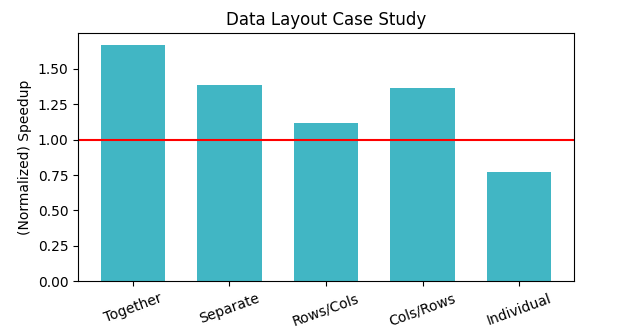
\includegraphics[width=0.9\linewidth]{figures/graphs/case_study.png}
    \caption{Speedups for the five data layout case studies (higher is better). Note that the second bar (``Separate'') corresponds to the leftmost bar of {\sf mm.3} in Figure~\ref{fig:vector-speedups}.}
    \Description{Bar graph showing speedup from vectorization for five data layout case studies}\label{fig:data-layout-case-study}
\end{figure}
\begin{figure}
    \centering
    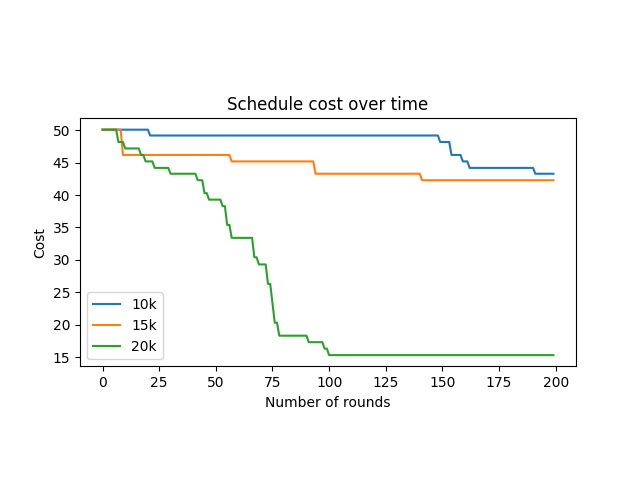
\includegraphics[width=0.9\linewidth]{figures/graphs/schedules.png}
    \vspace{-1em}
    \caption{\hl{Schedule cost over time (lower is better) for different numbers of simulated annealing iterations for data layout per step of scheduling.}}
    \Description{Multiple line graphs showing the schedule cost over time for different optimization parameters}\label{fig:schedule-cost}
\end{figure}


\subsection{Effects of Search and Co-Optimization}\label{sec:search-and-cooptimization}
% % \milind{bad section title :-) Call it something like ``Effects of Search and Co-optimization.'' There should be a research question in the intro that directly pertains to the results of this study}
% % \milind{Don't just launch into the figure description. Remind people why we're here :-)}\raghav{Is this better?}
\hl{We would like to know how effective {\system}'s schedule search strategy is, and in particular, how good of a job it does at optimizing data layout and schedule} {\em \hl{together}}.
\hl{To test this, we compile the 5-point distances benchmark with three different levels of data layout by varying the number of iterations of simulated annealing, and record the cost of the generated schedule during each round of the search.}

\hl{Figure~{\ref{fig:schedule-cost}} shows the cost of the vector schedule over time for various levels of data layout.
The blue line depicts the schedule cost when we use 10k iterations of simulated annealing to find an optimal data layout at each step; the orange line is 15k iterations and the green line is 20k iterations.
As expected, doing more iterations of simulated annealing has a large effect on the efficiency of the final schedule, since we rely heavily on the fact that the data layout being used to guide each round of the search is close to optimal.
In compiling all our benchmarks, we use 20k iterations of annealing (the green line).}

\subsection{Optimality Tradeoffs from Timeouts}\label{sec:ilp-ablation}
\hl{The synthesis procedure we use for generating the final (aligned) schedule from a pre-schedule uses iterative calls to an ILP solver that reduce the schedule height constraint until hitting a timeout.
This is to prevent the synthesis time from blowing up, but it does come at the cost of sacrificing some optimality, since the solver might time out before finding the smallest possible schedule. 
In this section, we investigate the extent to which this choice matters by instead using a version of the scheduler that directly finds the minimal-height schedule with no timeout. This approach guarantees that the synthesized schedules have minimal height.\footnote{Note that because the alignment algorithm cannot account for blend costs---they arise after alignment---the minimal {\em height} schedule may not be the minimal {\em cost} schedule.} Table~{\ref{tab:ilp-ablation}} summarizes the results. We see that compilation time increases with the optimal ILP, but speedups are comparable (sometimes faster, and even sometimes slower, due to different blends).}

\begin{table}
    \caption{\hl{Comparison of compilation time (seconds) and vectorization speedup with vs. without synthesis timeouts.}}\label{tab:ilp-ablation}
    \small
    \centering
    \begin{tabular}{lcccc}
        \toprule
        Benchmark & \multicolumn{2}{c}{Timeout} & \multicolumn{2}{c}{No Timeout}\\\cline{2-5}

         & Time & Speedup & Time & Speedup \\\midrule
        dist.5.un & 619 & 1.70 & 752 & 1.75 \\
        dist.5.partially & 629 & 1.73 & 751 & 1.76 \\
        dist.5.fully & 609 & 2.08 & 752 & 2.16 \\
        \midrule
        conv.4.2.un & 97 & 1.75 & 122 & 1.78 \\
        conv.4.2.partially & 80 & 3.12 & 102 & 3.19 \\
        conv.4.2.fully & 71 & 3.21 & 87 & 3.15 \\
        \midrule
        conv.5.3.un & 206 & 1.79 & 260 & 1.80 \\
        conv.5.3.partially & 211 & 2.48 & 261 & 2.57 \\
        conv.5.3.fully & 208 & 3.32 & 254 & 3.30 \\
        \midrule
        dot.3.un & 10 & 2.11 & 13 & 2.15 \\
        dot.3.partially & 10 & 2.11 & 13 & 2.13 \\
        dot.3.fully & 10 & 2.12 & 13 & 2.14 \\
        \midrule
        dot.6.un & 159 & 2.51 & 202 & 2.20 \\
        dot.6.partially & 154 & 2.51 & 193 & 2.21 \\
        dot.6.fully & 156 & 2.51 & 198 & 2.20 \\
        \midrule
        dot.10.un & 254 & 2.21 & 320 & 2.75 \\
        dot.10.partially & 257 & 2.15 & 323 & 2.77 \\
        dot.10.fully & 251 & 2.27 & 311 & 2.74 \\
        \bottomrule
    \end{tabular}
\end{table}

% The main tradeoff to be made here is one of compilation time: obviously, annealing for fewer iterations results in faster compilation, but worse schedules.
%\begin{figure}[t]
%\end{figure}


% We evaluate \system by compiling several computational kernels, of the sort that might be found in machine-learning code, and comparing their vectorized performance against an unvectorized (scalar) baseline implementation. Both the scalar and vector versions use the same FHE backend.
% Each of the matrix or vector inputs to the kernels are grouped into their own vectors as described in Section~\ref{sec:duplicating-inputs}.
%Although this can lead to worse schedules than if we didn't force groupings, we expect this to be the most common use case. \raghav{Is that what I wanna say? Or should I just combine it with the previous sentence and say ``yeah we force packings, yeah we know its not optimal.''}

% Each kernel is used in two benchmarks with differently sized inputs and three different replication strategies: once with both inputs replicated, once with only one input replicated, and once with neither input duplicated. 
% The exact benchmarks used are:
% \begin{itemize}
%     \item Matrix/Matrix multiply ($2 \times 2$ and $3 \times 3$)
%     \item Matrix/Matrix multiply followed by determinant ($2 \times 2$ and $3 \times 3$)
%     \item Pairwise distance computation (2 points and 3 points)
%     \item Vector dot product (vector size of 3 and 6)
%     \item Matrix convolution ($4 \times 4$ matrix with $2 \times 2$ kernel and $3 \times 3$ kernel)
% \end{itemize}

% % Figure~\ref{fig:ml-kernels} shows the performance results for these benchmarks.
% The red bars show the scalar execution time (normalized to 1), and the blue bars, the relative vector execution time (a smaller blue bar is better).
% Vector execution ranges from 0.77 to 6.2 times faster than scalar execution.
% Almost all benchmarks are substantially faster with vectorization, except those with lots of dependences (such as pairwise distance) or lots of reuse (such as matrix convolution), both of which result in a lot of data shuffling.

% % \milind{Start with the punchline -- don't keep people in suspense: vector execution ranges from $0.xxx$ to $y$ times faster than scalar execution. Almost all benchmarks, except those with ... have substantially faster vector than scalar runtimes, and performing full replication, which means less rotation is needed, is uniformly faster -- up to 5 times faster. Once you give them the punchline, then you can explain the rest of the details.}

% % Most of our benchmarks see a greater speedup from vectorization as we move from unreplicated inputs to fully replicated inputs.
% % This is what we expect, because, as discussed in Section~\ref{sec:duplicating-inputs}, replicating a set of inputs leads to fewer rotations necessary to get each of them to the correct lanes.
% % Performing full replication ameliorates these problems (Section~\ref{sec:duplicating-inputs}), and is uniformly faster.
% Fully-replicated vector benchmarks range from a 6.2$\times$ speedup for \texttt{mat\_mul2x2}, to an approximately $25\%$ speedup for \texttt{mat\-\_mul\-\_det3x3}

% In the unreplicated runs, we see some of the vectorized kernels (\texttt{mat\-\_convol\-\_4x4x2x2}, \texttt{mat\-\_mul\-\_det3x3}, and \texttt{pair\-wise\-\_dist2x2}) are actually {\em slower} than the scalar baseline.
% This is because the overhead of all the rotations these benchmarks incur outweighs any benefits gained from vectorization.
% In fact, it makes sense that these benchmarks would behave like that: convolution is a computation with substantial data reuse, leading to a high number of rotations to move data.
% The $2 \times 2$ pairwise distance benchmark has a fully-connected dependence graph, leading to essentially the worst case scenario for vectorization.
% And computing the determinant at the end of \texttt{mat\_mul\_det3x3} requires a reduction of 9 values, with no symmetries between them to exploit.
% However, even in these examples, the vectorized code is no more than 20\% worse than scalar, showing that despite the high rotation costs, \system is still able to properly take advantage of vectorization opportunities.
% %\raghav{This all kind of seems like a jumble but I hope I'm getting the point across}

% Overall, we see that it is almost always better to fully replicate inputs when vectorizing, unless specifically compiling several composable kernels separately. While it may seem that replicating data could increase overheads (e.g., by requiring more time to encrypt the input, or by requiring larger vector widths), in practice it does not. Encryption is vectorized in the same way as computation so does not take appreciably longer if the same data is encrypted multiple times. And vector widths in FHE are very high to begin with, so there is ample lane space to house the replicated data.

% Visually inspecting the vector code generated by \system reveals that it often automatically finds what known optimal schedules.
% For example, in the dot product kernels, \system first packs all of the multiplications into a single vector operation, then vectorizes the levels of the logarithmic reduction tree.\footnote{Note that the logarithmic reduction tree arises because the eDSL implementation of dot product uses a recursive sum operation---\system does not introduce new parallelism. Nevertheless, \system correctly exploits the parallelism that {\em does} exist in the circuit.}
% In the \texttt{mat\_mul\_det} kernels, \system first identifies the the highly vectorizable matrix multiply part of the computation, vectorizes that, and then essentially computes the highly irregular determinant on a single lane.

% \milind{Add a discussion here about visually inspecting the generated code, and point out where and whether coyote does especially cool stuff, or where it breaks down.}


% \subsection{Fuzzed Microbenchmarks}
% To investigate how various aspects of program structure affect \system's ability to vectorize, we randomly generate several expression trees according to three regimes:
% \begin{enumerate}
%     \item {\em Sparse}: Many operations have one leaf node input, the tree is not very balanced
%     \item {\em Dense, homogeneous}: The expression tree is both full and complete, and all the operations are isomorphic
%     \item {\em Dense, nonhomogeneous}: The expression tree is both full and complete, each operation has a 50/50 chance of being an add or a multiply.
% \end{enumerate}
% We generate ten trees for each regime: five with a maximum depth of 3, and five with a maximum depth of 6.
% % The relative speedups for these trees are shown in Figure~\ref{fig:fuzzed-trees}.
% We see that aside from the sparse trees of depth 3, all the rest show speedups when vectorizing, which makes sense since the sparse computations tend to be much more linear and have fewer opportunities for vectorization.
% The depth 3 trees show on average less speedup than the depth 6 trees, since they also have less work available to vectorize, and less parallelism in their circuits. %\raghav{Is this true? I'm basically trying to say that the scalar is already not bad for a tiny tree so what's the point in vectorizing it}\milind{It's basically about less parallelism. For a complete tree, parallelism is n/log(n), so as n gets bigger, there is more parallelism --- a depth 6 tree has 4 times as much parallelism as a depth 3 tree}

% \begin{figure}
%     % 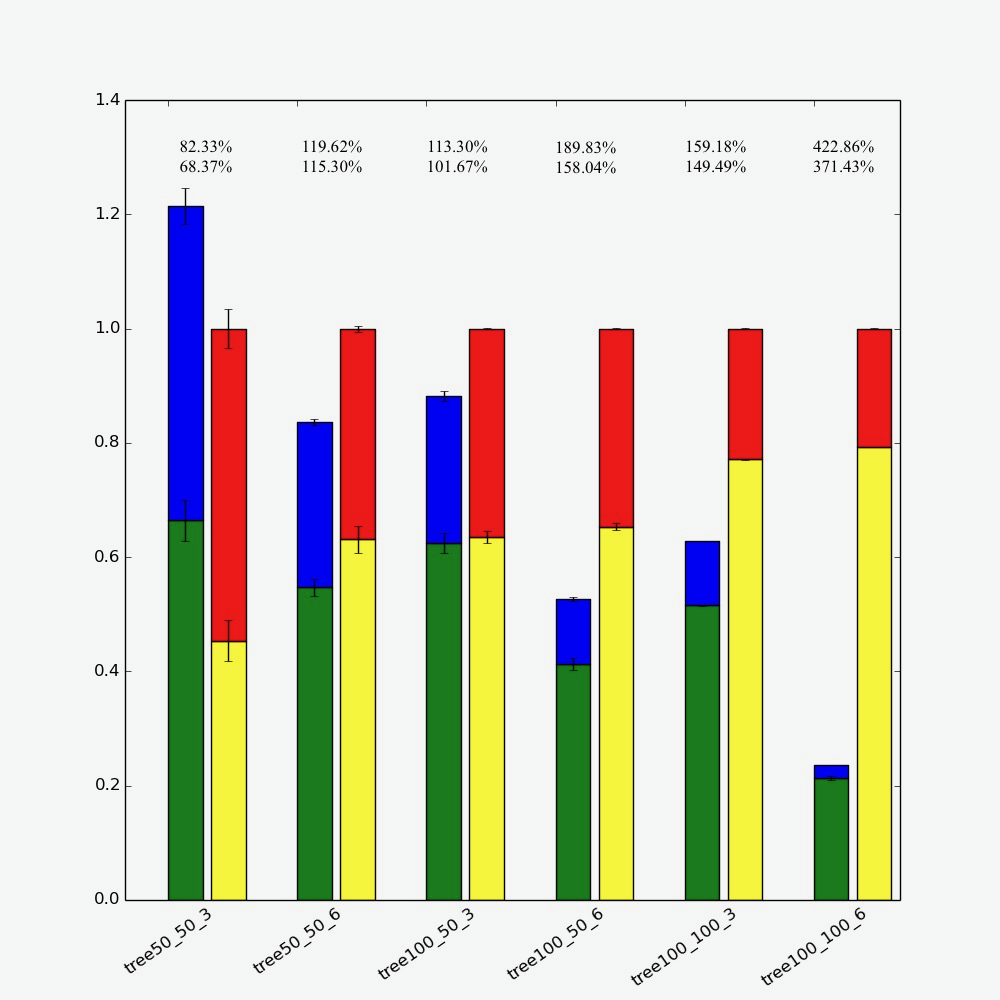
\includegraphics[width=0.9\columnwidth]{figures/graphs/TreeGraphwithNumbers.png}
%     \vspace{-0.5em}
%     \caption{Vectorization speedups on microbenchmarks. Blue/green bars represent vector time, and red/yellow bars represent (normalized) scalar time, with a smaller blue/green bar being better. Bars are split between time execution time and encryption time, with execution time on the bottom (green and yellow) and encryption time on top (blue and red). The numbers on top of the bars represent the speedup of vector over scalar, with the first one including encryption time and the second one excluding it.}\label{fig:fuzzed-trees}
% \end{figure}
\section{Related Work}\label{sec:related-work}
There are two main categories of related work. This section first discusses work on FHE vectorization, and then discusses more general approaches to plaintext vectorization 
%\raghav{Your favorite part: finding a better way to taxonomize all of these!}

\subsection{Compilation and Vectorization for FHE}
Prior work has been done on building vectorizing compilers for FHE applications \cite{CHET, Porcupine}.
CHET \cite{CHET} is a vectorizing compiler for homomorphic tensor programs that automatically selects encryption parameters, and chooses optimal data layout strategies.
CHET is specifically targeted towards optimizing the dense tensor computations in neural network inference, and does not apply to a broader class of programs, especially those with irregular computations that are not so easily vectorized.
\system makes no assumptions about the domain of the program, and can vectorize even highly irregular computations.

Porcupine~\cite{Porcupine} is a vectorizing compiler that uses a sketch-based synthesis approach to generate vectorized kernels given a reference implementation. While Porcupine is more general than CHET, it relies on programmers providing partial implementations in the form of sketches, making it less automatic than Coyote. Furthermore, Porcupine relies on the sketches to constrain the search space of rotations, while Coyote is specifically designed to reduce the number of rotations.

%Porcupine \cite{Porcupine} is another vectorizing compiler that uses a synthesis-based approach to automatically generate vectorized FHE kernels given a reference implementation.
%Porcupine is more general than CHET, but it is still mostly targeted towards regular, easily vectorizable computations.
%While Porcupine can, in theory, generate kernels for any computation, its treatment of rotations makes it harder to adapt to vectorizing irregular programs.
%Porcupine considers rotations directly as inputs to arithmetic expressions, and relies on a sketch to constrain the search space and a solver to find programs with optimal performance characteristics.
%Irregular applications without many apparent symmetries to exploit incur many asymmetric rotations, making it more difficult for the solver to produce an optimal schedule. The search space becomes prohibitively large, and is not tuned towards finding minimal sets of rotations.
%In contrast, because \system focuses on limiting rotations, its schedule search prioritizes vector schedules that {\em specifically} reduce the number of required rotations.
%% \raghav{Maybe another thing to say (emphasize?) is that the \system and Porcupine approaches are fundamentally different in that the latter relies on a sketch to synthesize good schedules while \system finds them automatically.}
%
%Additionally, Porcupine's synthesis-based approach results in very long compile times for programs with more than a few instructions.
%Their solution to this problem is to break large programs into multiple smaller, composable kernels and synthesize solutions to each kernel independently.
%This has two major drawbacks: First, the burden of decomposing the program falls on the programmer. Second, synthesizing kernels separately means that Porcupine is unable to find optimizations across kernel boundaries, so a poor decomposition can preclude a more efficient vectorization.
%\system, on the other hand, can compile much larger programs in a reasonable amount of time, and the circuit quotienting strategy automatically breaks large programs up into smaller sequences of vectorizable instructions. %\raghav{TODO: add instruction counts to the eval?}

%\raghav{I think I explained that correctly?}\milind{Sounds good.}

Gazelle \cite{Gazelle} is a framework for secure neural network inference in FHE.
While it is very optimized for a particular use case, Gazelle is not {\em general}: it consists of a library of highly efficient vectorized kernels that are useful in neural network applications.
By contrast, \system can take arbitrary kernels and generate efficient vectorized code on the fly. %\raghav{Not sure how to put this nicely, actually.}

Lee, et. al \cite{CircuitRewriting} describe a general method for automatically rewriting arithmetic and boolean FHE circuits according to a cost model by learning semantically sound rewrite rules.
This approach explores the space of scalar rewrites but does not directly deal with vectorization, making it orthogonal to ours: a technique like this could first be applied to an arbitrary computation to transform it into one more amenable to vectorization before applying \system.

One class of related work consists of compilers \cite{Ramparts, ALCHEMY, EVA, Cingulata} that automatically lift programs written in a high level DSL into optimized FHE circuits that perform the same computation.
Unlike \system, these circuit optimizations do not include automatic vectorization. Although ACLHEMY~\cite{ALCHEMY} and EVA~\cite{EVA} \textit{do} support ciphertext packing, they require the programmer to perform the vectorization.
%\raghav{Remove this since I folded EVA into the (ramparts, alchemy, etc.) sentence earlier?}
%Encrypted Vector Arithmetic (EVA) \cite{EVA} is another Python DSL that aims to make FHE programming more accessible; in particular, it also supports writing vector computation.
%However, unlike \system, EVA requires the programmer to write vectorized code directly: it does not support automatically vectorizing arbitrary kernels.
%\raghav{Mention that EVA automatically does parameter selection? Or the fact that we could potentially target EVA as a backend if it weren't restricted to CKKS?}\milind{nah.}

\subsection{General Purpose Vectorization in non-FHE Settings}
Superword-Level Parallelism is a technique for automatically vectorizing programs~\cite{SLP}.
SLP iterates over a sequence of scalar instructions and computes ``vector packs,'' or sets of isomorphic instructions that can be packed together into vectors.
Because SLP does not rely on the presence of data-parallel structures like loops to aid in vectorization, it works well even for irregular programs.
When computing vector packs, SLP does not account for how expensive rotations are in FHE, leading to schedules with very high data shuffling costs. 

VeGen \cite{VeGen} is a recent variant of SLP, introducing a notion of {\em lane level parallelism} that reasons about which lanes are performing which computations, allowing it to reason about rotation costs when building vector packs.
For example, VeGen can reason about the rotation costs to pack together operands for an instruction into a temporary vector, and can use this to decide whether or not packing those instructions is worth it.
However, this reasoning only happens locally, and VeGen does not incorporate information about how instruction packing might affect rotations much later in the program.

%\raghav{Spotcheck again?}
goSLP \cite{goSLP} reasons about globally optimal packing, and finds lane placements that minimize data shuffling costs. 
However, there are assumptions baked into its cost model that make it fundamentally unsuitable for the FHE setting.
goSLP frames vectorization overhead in terms of the number of {\em pack} and {\em unpack} operations incurred.
For example, permuting the slots of a single vector incurs one unpack, whereas blending the contents of N vectors (without any permutation) incurs N unpacks.
This cost model implicitly requires wide blends to be more expensive than arbitrary permutations, almost the opposite of FHE's cost model. In FHE, blends are almost free (instantiated as cheap plaintext multiplies and ciphertext adds) whereas a ``bad'' permutation can require O(n) rotates to realize.
% In other words, in the FHE world, there are often highly profitable schedules that require many blends and few rotates, but the framing goSLP uses for vectorization overhead will cause it to forego these schedules for more conservative ones.
In other words, goSLP will often forego a highly profitable schedule with many blends and few rotates, and instead opt for a more conservative one.    
Additionally, goSLP does lane placement (permutation selection) {\em after} finding vector packs, creating situations like the one described in Section~\ref{sec:intro} in which the ostensibly profitable packing does not admit a good data layout.
By contrast, \system's cooperative scheduling strategy ensures that this does not happen.

% While goSLP does reason globally about lane placement, it has two drawbacks in an FHE context. First, it packs instructions into vectors before considering shuffling costs, so may over-aggressively vectorize, while \system may forego some vectorization opportunities in the name of getting packing larger expressions without rotation. Second, its lane placement algorithm considers arbitrary permutations, which are impractically expensive in FHE.
% \raghav{goSLP frames vectorization overhead in terms of the number of {\em pack} and {\em unpack} operations incurred. For example, permuting the slots of a single vector incurs one unpack, whereas blending the contents of N vectors (without any permutation) incurs N unpacks. In other words, goSLP bakes in the assumption that wide blends are much more expensive than arbitrary permutations. This is fundamentally incompatible with FHE, since blends are almost free, whereas bad permutations can require several expensive rotations to realize. Essentially, in the FHE world, its often better to produce a schedule that {\em looks much worse} than to produce the traditionally optimal one.}

% \raghav{Can you check how this is worded?}
There is a class of work that deals specifically with optimizing permutations in vectorized code~\cite{SIMDPermutations,SIMDAlignment,SwizzleInventor}. 
Ren, et. al~\cite{SIMDPermutations} present an algebra for reasoning about and reducing the permutation workload in SIMD programs.
Eichenberger, et. al~\cite{SIMDAlignment} develop a technique to efficiently realign memory accesses produced as a result of vectorizing a loop.
Finally, Swizzle Inventor~\cite{SwizzleInventor} is a system which automatically synthesizes efficient data movement kernels for vectorized GPU code.
The primary obstacle \system faces in directly applying these approaches is that they tackle the data movement problem {\em after the kernel has been vectorized}.
As we discussed earler, in the world of FHE, packing and data movemnt are problems that must be reasoned about together.
There are two additional drawbacks: Eichenberger, et. al focus on aligning memory accesses in regular, data-dense loops, but this is not the setting in which Coyote operates.
In the case of Swizzle Inventor, the sketches it uses to guide synthesis rely on efficiently accessing arbitrary slots of a packed vector, which is not possible in FHE without incurring significant rotation overheads.


% There is a class of work that deals specifically with optimizing permutations in vectorized code~\cite{SIMDAlignment,SIMDPermutations,SwizzleInventor}, the most recent of which is Swizzle Inventor~\cite{SwizzleInventor}, a system which automatically synthesizes efficient data movement kernels for vectorized GPU code.
% % Swizzle Inventor \cite{SwizzleInventor} is a system which automatically synthesizes efficient data movement kernels for vectorized GPU code.
% There are two primary obstacles \system faces in directly applying this sort of approach to our setting.
% First, these works tackle the data movement problem {\em after the kernel has been vectorized}. As we discussed earlier, in the world of FHE, packing and data movement are problems that must be reasoned about together.
% Second, in the case of Swizzle Inventor, the sketches it uses to guide its synthesis rely on efficiently accessing arbitrary slots of a packed vector. However, this is not possible with FHE vectors without incurring significant rotation overheads.

Diospyros~\cite{Diospyros} is an equality saturation--based vectorization strategy that constructs an e-graph~\cite{EqualitySaturation, egg} of programs that are semantically equivalent to a given specification, and then uses a custom cost model to extract an efficient vector program, together with necessary shuffles.
The simplicity of the cost model it associates to various shuffles makes it unsuitable to deal with the peculiarities and inflexibility of FHE rotations.

%By reasoning globally about the entire dependence graph of the program at once, \system can identify such phenomena when making vector packs.
%\system can also automatically find vector schedules that are amenable to more efficient data movement, and can propagate this information back through the program this to identify more optimal data layouts.

% Talk about SLP
% Talk about FHE (Gentry paper)
% Talk in depth about CHET
% Talk in depth about Porcupine
\section{Conclusion}\label{sec:conclusion}
This paper presented \system, the first vectorizing compiler for arbitrary FHE programs that considers FHE's unique cost model for data movement when vectorizing.
\system operates at a coarser level than most vectorizers, allowing it to minimize the data movement overhead of vectorizing by only packing together sufficiently similar subexpressions.
\system can also find optimal lane placement and data layouts that encourage more efficient rotation patterns.
\system can automatically vectorize a large class of useful kernels, showing speedups of up to 3.5$\times$ over scalar code.

%Potential avenues for future work include fine-tuning \system's cost model and adding semantics-preserving transformations that can restructure circuits to be more vectorizable.
\section*{Acknowledgements}
The authors appreciate the feedback from anonymous reviewers from PLDI 2022, OOPSLA 2022 and ASPLOS 2023 that have improved the paper.
This work was  partially supported by NSF grants CCF-1908504 and CCF-1919197, as well as Cisco.
% \pagebreak
\appendix
\section{Artifact Appendix}

%%%%%%%%%%%%%%%%%%%%%%%%%%%%%%%%%%%%%%%%%%%%%%%%%%%%%%%%%%%%%%%%%%%%%
\subsection{Abstract}

The artifact contains everything necessary to replicate the results of this paper, including:
\begin{itemize}
    \item An implementation of the compiler described in the paper
    \item A backend test harness for profiling the vectorized code Coyote generates
    \item Implementations of all the benchmarks used in the evaluation
    \item Various scripts necessary to automate the process of compiling, running, and collecting data from the benchmarks.
\end{itemize}

Note that there are two experiments omitted from the artifact, as they require nontrivial manual effort to set up and run. These are the {\tt mm.16.blocked} benchmark described in Section~\ref{sec:scalability}, and Figure~\ref{fig:schedule-cost}

\subsection{Artifact check-list (meta-information)}

{\small
\begin{itemize}
  \item {\bf Compilation: } Translates a python program into an arithmetic circuit, vectorizes it, and generates C++ FHE code
  \item {\bf Transformations: } Loop unrolling, function inlining, circuit vectorization
  \item {\bf Experiments: } Compiling real-world benchmarks, compiling randomly generated polynomial programs, experimenting with data layouts
  \item {\bf How much disk space required (approximately)?: } 200MB
  \item {\bf How much time is needed to complete experiments (approximately)?: } 45 minutes - 1 hour for the small version, up to several hours for running all the benchmarks
  \item {\bf Publicly available?: } Yes
  \item {\bf Code licenses (if publicly available)?: } MIT
  \item {\bf Archived (provide DOI)?: } 10.5281/zenodo.7591603 or https://github.com/raghav198/coyote
  
\end{itemize}
}

%%%%%%%%%%%%%%%%%%%%%%%%%%%%%%%%%%%%%%%%%%%%%%%%%%%%%%%%%%%%%%%%%%%%%
\subsection{Description}

\subsubsection{How to access}

{\em Obligatory}

\subsubsection{Hardware dependencies}
No specialized hardware is required to use Coyote, beyond whatever may be necessary to efficiently run z3 and SEAL.

\subsubsection{Software dependencies}
\begin{itemize}
    \item The {\tt coyote} compiler is implemented in Python 3.10 and uses the networkx and z3 modules for its analysis
    \item The test harness backend is written in C++ and uses version 3.7 of the Microsoft SEAL library for its FHE implementation
    \item The test harness uses cmake for its build system
\end{itemize}

%%%%%%%%%%%%%%%%%%%%%%%%%%%%%%%%%%%%%%%%%%%%%%%%%%%%%%%%%%%%%%%%%%%%%
\subsection{Installation}

The Dockerfile provided with the artifact automatically builds and installs all dependencies of Coyote. To build and run the Docker image, run the following commands from the directory containing the Dockerfile:

\begin{minted}{Bash}
    $ docker build -t coyote .
    $ docker run -it coyote bash
\end{minted}

%%%%%%%%%%%%%%%%%%%%%%%%%%%%%%%%%%%%%%%%%%%%%%%%%%%%%%%%%%%%%%%%%%%%%
\subsection{Experiment workflow}
This section describes a workflow to reproduce a subset of the results in the paper.
We've recorded the approximate time it takes to complete each step inside the Docker image on a 2020 M1 MacBook Air.
Lets start by building all the {\tt small} benchmarks (all replication sorts for {\tt conv.4.2}, {\tt mm.2}, {\tt dot.3}, {\tt dot.6}, and {\tt dot.10}, as well as the ungrouped {\tt sort[3]}). 
% 13 minutes
\begin{minted}{Bash}
    $ python3 compile_benchmarks.py --preset small    
\end{minted}
We can also build the data layout case study from Section~\ref{sec:data-layout} of the paper, although note that these circuits are considerably larger, so compiling them will take some time:
% 15 minutes
\begin{minted}{Bash}
    $ python3 compile_benchmarks.py --preset layout    
\end{minted}
Lets also build some of the polynomial trees; in particular, we'll build two of the depth 5 trees in each of the three regimes.
% 5 minutes
\begin{minted}{Bash}
    $ python3 polynomial_benchmarks.py -d 5 -r \
    "100-100" "100-50" "50-50" -i 2    
\end{minted}

We can see, for example, some of the Coyote vector IR:
\begin{minted}{Bash}
    $ cat sort_3/vec    
\end{minted}
and the corresponding generated vector C++ code:
\begin{minted}{Bash}
    $ cat bfv_backend/coyote_out/sort_3/vector.cpp    
\end{minted}

To build {\em all} the benchmarks from the paper (small, medium, and large, as well as the layouts and the random polynomials), run the following instead of following the above steps:
\begin{minted}{Bash}
    $ python3 coyote_compile.py benchmarks.py -c "*"
    $ python3 polynomial_benchmarks.py -d 5 10 -r \
        "100-100" "100-50" "50-50" -i 5    
\end{minted}
However, this is not recommended and will take several hours to complete, as several of the circuits being compiled are quite large.

Now, we need to compile all the C++ code and collect data. Although we used 50 runs and 50 iterations in the paper, lets only use 10 of each to make this go faster:
% compile: % compile+run: 13 minutes
\begin{minted}{Bash}
    $ python3 build_and_run_all.py --runs 10 --iters 10    
\end{minted}
You should see some CMake output followed by the encryption and run times for both scalar and vector versions of each circuit. Note that this script will not re-run benchmarks that already have corresponding CSV files in {\tt bfv\_backend/csvs/}.
Once this is finished running, we can look at one of the generated CSV files:
\begin{minted}{Bash}
    $ cat bfv_backend/csvs/sort/sort_3.csv    
\end{minted}
Now that we've collected all the data for these benchmarks, we can generate the graphs:
\begin{minted}{Bash}
    $ python3 figures.py
\end{minted}
This will generate three plots: vector\_speedups.png, case\_study.png, and trees.png. To view these, either attach to the running Docker container (e.g. using VS Code), or copy the files to your host machine:
\begin{minted}{Bash}
    $ docker cp $(docker ps -q):/home/artifact/graphs/ .    
\end{minted}

Compiling all the small benchmarks takes about 13 minutes, generating and compiling the random polynomial benchmarks takes about 5 minutes, compiling the data layout case study takes about 15 minutes, and building and running all the benchmarks takes about 15 minutes.


%%%%%%%%%%%%%%%%%%%%%%%%%%%%%%%%%%%%%%%%%%%%%%%%%%%%%%%%%%%%%%%%%%%%%
\subsection{Evaluation and expected results}

After running through the workflow described above, you should have generated three plots, each of which replicates part of the experiments in this paper:
\begin{itemize}
    \item {\tt vector\_speedups.png} corresponds to Figure~\ref{fig:vector-speedups}
    \item {\tt trees.png} corresponds to Figure~\ref{fig:polynomial-speedups}
    \item {\tt case\_study.png} corresponds to Figure~\ref{fig:data-layout-case-study}
\end{itemize}
Note that the generated graphs may not contain all the experiments found in the paper (for example, not all the benchmarks in Figure~\ref{fig:vector-speedups} are built in the above workflow, and neither are the depth 10 trees in Figure~\ref{fig:polynomial-speedups}, as these take a long time to compile).
However, the speedups should resemble those in the corresponding figures.

%%%%%%%%%%%%%%%%%%%%%%%%%%%%%%%%%%%%%%%%%%%%%%%%%%%%%%%%%%%%%%%%%%%%%
\subsection{Experiment customization}
\subsubsection{Writing a Coyote program}
Coyote is a DSL embedded in Python, so Coyote programs are just Python functions. To tag a function as a circuit for Coyote to compile, first get an instance of the Coyote compiler:
\begin{minted}{Python}
    from coyote import *
    coyote = coyote_compiler()
\end{minted}
Next, use the compiler to annotate your function with input types:
\begin{minted}{Python}
@coyote.define_circuit(A=matrix(3, 3), B=matrix(3, 3))
def matrix_multiply(A, B):
    ...
\end{minted}
For a full discussion of the available types and their compile-time semantics, see Section~\ref{sec:surface-language}
Finally, use the build script {\tt coyote\_compile.py} to invoke the Coyote compiler on the Python file in which this code is saved:
\begin{minted}{Bash}
    python3 coyote_compile.py circuits.py -c \
        matrix_multiply
\end{minted}
\subsubsection{Invoking the Compiler}
The Coyote compiler can be invoked from the command line via {\tt coyote\_compile.py}. The example invocation above does the following:
\begin{enumerate}
    \item It parses {\tt circuits.py} and loads a list of all circuits defined in that file
    \item It uses Coyote to compile/vectorize the specified {\tt matrix\_multiply} circuit
    \item It creates a directory called {\tt matrix\_multiply} and saves intermediate scalar and vector code into that directory
    \item It lowers the intermediate code into C++ and saves it in {\tt bfv\_backend}
\end{enumerate}
The script expects the name of a Python file that defines one or more circuits (as described above), and then takes a number of command-line parameters:
\begin{itemize}
    \item {\tt -l}, {\tt --list}: Lists all the circuits defined in the file and exit, does not actually compile anything
    \item {\tt -c}, {\tt --circuits}: Load the specified circuits from the file and compile them into C++
    \item {\tt -o}, {\tt --output-dir}: Specify the directory into which to place the generated intermediate code (defaults to the directory from which coyote\_compile.py is invoked)
    \item {\tt --backend-dir}: Specify the directory containing the test harness backend (defaults to bfv\_backend/)
    \item {\tt --no-cpp}: Stops after generated the intermediate code and doesn't generate C++
    \item {\tt --just-cpp}: Uses pregenerated intermediate code to generate C++ instead of recompiling the circuit; this fails if it can't find the intermediate code under [output-dir]/[circuit-name]/
\end{itemize}
\subsubsection{Running the test harness}
The backend test harness comes with a CMake file that automatically builds binaries for everything under {\tt coyote\_out/}. The generated binaries perform a number of runs, where each run consists of executing the scalar and vectorized circuits on random encrypted inputs for a number of iterations and then outputting the total time each version (scalar and vector) took to encrypt, as well as run. All these outputs are then saved into a csv file with the same name as the circuit (e.g. running the binary generated from the example above would create a file called {\tt matrix\_multiply.csv}).

The number of runs and iterations default to 50 each (as these are the values used in this paper), but are configurable via cmake. An example invocation that uses 10 runs with 10 iterations each is as follows:

\begin{minted}{Bash}
    $ mkdir bfv_backend/build
    $ cd bfv_backend/build
    $ cmake .. -DRUNS=10 -DITERATIONS=10
    $ make -j16
\end{minted}
%%%%%%%%%%%%%%%%%%%%%%%%%%%%%%%%%%%%%%%%%%%%%%%%%%%%%%%%%%%%%%%%%%%%%
\subsection{Methodology}

Submission, reviewing and badging methodology:

\begin{itemize}
  \item \url{https://www.acm.org/publications/policies/artifact-review-badging}
  \item \url{http://cTuning.org/ae/submission-20201122.html}
  \item \url{http://cTuning.org/ae/reviewing-20201122.html}
\end{itemize}

% \pagebreak
% \clearpage
% \onecolumn
% \begin{multicols}{2}
    % \balance
\bibliographystyle{ACM-Reference-Format}
%%% -*-BibTeX-*-
%%% Do NOT edit. File created by BibTeX with style
%%% ACM-Reference-Format-Journals [18-Jan-2012].

\begin{thebibliography}{24}

  %%% ====================================================================
  %%% NOTE TO THE USER: you can override these defaults by providing
  %%% customized versions of any of these macros before the \bibliography
  %%% command.  Each of them MUST provide its own final punctuation,
  %%% except for \shownote{}, \showDOI{}, and \showURL{}.  The latter two
  %%% do not use final punctuation, in order to avoid confusing it with
  %%% the Web address.
  %%%
  %%% To suppress output of a particular field, define its macro to expand
  %%% to an empty string, or better, \unskip, like this:
  %%%
  %%% \newcommand{\showDOI}[1]{\unskip}   % LaTeX syntax
  %%%
  %%% \def \showDOI #1{\unskip}           % plain TeX syntax
  %%%
  %%% ====================================================================
  
  \ifx \showCODEN    \undefined \def \showCODEN     #1{\unskip}     \fi
  \ifx \showDOI      \undefined \def \showDOI       #1{#1}\fi
  \ifx \showISBNx    \undefined \def \showISBNx     #1{\unskip}     \fi
  \ifx \showISBNxiii \undefined \def \showISBNxiii  #1{\unskip}     \fi
  \ifx \showISSN     \undefined \def \showISSN      #1{\unskip}     \fi
  \ifx \showLCCN     \undefined \def \showLCCN      #1{\unskip}     \fi
  \ifx \shownote     \undefined \def \shownote      #1{#1}          \fi
  \ifx \showarticletitle \undefined \def \showarticletitle #1{#1}   \fi
  \ifx \showURL      \undefined \def \showURL       {\relax}        \fi
  % The following commands are used for tagged output and should be
  % invisible to TeX
  \providecommand\bibfield[2]{#2}
  \providecommand\bibinfo[2]{#2}
  \providecommand\natexlab[1]{#1}
  \providecommand\showeprint[2][]{arXiv:#2}
  
  \bibitem[Archer et~al\mbox{.}(2019)]%
          {Ramparts}
  \bibfield{author}{\bibinfo{person}{David~W. Archer},
    \bibinfo{person}{Jos\'{e}~Manuel Calder\'{o}n~Trilla}, \bibinfo{person}{Jason
    Dagit}, \bibinfo{person}{Alex Malozemoff}, \bibinfo{person}{Yuriy Polyakov},
    \bibinfo{person}{Kurt Rohloff}, {and} \bibinfo{person}{Gerard Ryan}.}
    \bibinfo{year}{2019}\natexlab{}.
  \newblock \showarticletitle{RAMPARTS: A Programmer-Friendly System for Building
    Homomorphic Encryption Applications}. In
    \bibinfo{booktitle}{\emph{Proceedings of the 7th ACM Workshop on Encrypted
    Computing \& Applied Homomorphic Cryptography}} (London, United Kingdom)
    \emph{(\bibinfo{series}{WAHC'19})}. \bibinfo{publisher}{Association for
    Computing Machinery}, \bibinfo{address}{New York, NY, USA},
    \bibinfo{pages}{57–68}.
  \newblock
  \showISBNx{9781450368292}
  \urldef\tempurl%
  \url{https://doi.org/10.1145/3338469.3358945}
  \showDOI{\tempurl}
  
  
  \bibitem[Brakerski et~al\mbox{.}(2012)]%
          {BrakerskiPacking}
  \bibfield{author}{\bibinfo{person}{Zvika Brakerski}, \bibinfo{person}{Craig
    Gentry}, {and} \bibinfo{person}{Shai Halevi}.}
    \bibinfo{year}{2012}\natexlab{}.
  \newblock \bibinfo{title}{Packed Ciphertexts in LWE-based Homomorphic
    Encryption}.
  \newblock
  \newblock
  
  
  \bibitem[Carpov et~al\mbox{.}(2015)]%
          {Cingulata}
  \bibfield{author}{\bibinfo{person}{Sergiu Carpov}, \bibinfo{person}{Paul
    Dubrulle}, {and} \bibinfo{person}{Renaud Sirdey}.}
    \bibinfo{year}{2015}\natexlab{}.
  \newblock \showarticletitle{Armadillo: A Compilation Chain for Privacy
    Preserving Applications}. In \bibinfo{booktitle}{\emph{Proceedings of the 3rd
    International Workshop on Security in Cloud Computing}} (Singapore, Republic
    of Singapore) \emph{(\bibinfo{series}{SCC '15})}.
    \bibinfo{publisher}{Association for Computing Machinery},
    \bibinfo{address}{New York, NY, USA}, \bibinfo{pages}{13–19}.
  \newblock
  \showISBNx{9781450334471}
  \urldef\tempurl%
  \url{https://doi.org/10.1145/2732516.2732520}
  \showDOI{\tempurl}
  
  
  \bibitem[Chen et~al\mbox{.}(2021)]%
          {VeGen}
  \bibfield{author}{\bibinfo{person}{Yishen Chen}, \bibinfo{person}{Charith
    Mendis}, \bibinfo{person}{Michael Carbin}, {and} \bibinfo{person}{Saman
    Amarasinghe}.} \bibinfo{year}{2021}\natexlab{}.
  \newblock \showarticletitle{VeGen: A Vectorizer Generator for SIMD and Beyond}.
    In \bibinfo{booktitle}{\emph{Proceedings of the 26th ACM International
    Conference on Architectural Support for Programming Languages and Operating
    Systems}} (Virtual, USA) \emph{(\bibinfo{series}{ASPLOS 2021})}.
    \bibinfo{publisher}{Association for Computing Machinery},
    \bibinfo{address}{New York, NY, USA}, \bibinfo{pages}{902–914}.
  \newblock
  \showISBNx{9781450383172}
  \urldef\tempurl%
  \url{https://doi.org/10.1145/3445814.3446692}
  \showDOI{\tempurl}
  
  
  \bibitem[Cowan et~al\mbox{.}(2021)]%
          {Porcupine}
  \bibfield{author}{\bibinfo{person}{Meghan Cowan}, \bibinfo{person}{Deeksha
    Dangwal}, \bibinfo{person}{Armin Alaghi}, \bibinfo{person}{Caroline Trippel},
    \bibinfo{person}{Vincent~T. Lee}, {and} \bibinfo{person}{Brandon Reagen}.}
    \bibinfo{year}{2021}\natexlab{}.
  \newblock \showarticletitle{Porcupine: A Synthesizing Compiler for Vectorized
    Homomorphic Encryption}. In \bibinfo{booktitle}{\emph{Proceedings of the 42nd
    ACM SIGPLAN International Conference on Programming Language Design and
    Implementation}} (Virtual, Canada) \emph{(\bibinfo{series}{PLDI 2021})}.
    \bibinfo{publisher}{Association for Computing Machinery},
    \bibinfo{address}{New York, NY, USA}, \bibinfo{pages}{375–389}.
  \newblock
  \showISBNx{9781450383912}
  \urldef\tempurl%
  \url{https://doi.org/10.1145/3453483.3454050}
  \showDOI{\tempurl}
  
  
  \bibitem[Crockett et~al\mbox{.}(2018)]%
          {ALCHEMY}
  \bibfield{author}{\bibinfo{person}{Eric Crockett}, \bibinfo{person}{Chris
    Peikert}, {and} \bibinfo{person}{Chad Sharp}.}
    \bibinfo{year}{2018}\natexlab{}.
  \newblock \showarticletitle{ALCHEMY: A Language and Compiler for Homomorphic
    Encryption Made EasY}. In \bibinfo{booktitle}{\emph{Proceedings of the 2018
    ACM SIGSAC Conference on Computer and Communications Security}} (Toronto,
    Canada) \emph{(\bibinfo{series}{CCS '18})}. \bibinfo{publisher}{Association
    for Computing Machinery}, \bibinfo{address}{New York, NY, USA},
    \bibinfo{pages}{1020–1037}.
  \newblock
  \showISBNx{9781450356930}
  \urldef\tempurl%
  \url{https://doi.org/10.1145/3243734.3243828}
  \showDOI{\tempurl}
  
  
  \bibitem[Dathathri et~al\mbox{.}(2020)]%
          {EVA}
  \bibfield{author}{\bibinfo{person}{Roshan Dathathri},
    \bibinfo{person}{Blagovesta Kostova}, \bibinfo{person}{Olli Saarikivi},
    \bibinfo{person}{Wei Dai}, \bibinfo{person}{Kim Laine}, {and}
    \bibinfo{person}{Madan Musuvathi}.} \bibinfo{year}{2020}\natexlab{}.
  \newblock \showarticletitle{EVA: An Encrypted Vector Arithmetic Language and
    Compiler for Efficient Homomorphic Computation}. In
    \bibinfo{booktitle}{\emph{Proceedings of the 41st ACM SIGPLAN Conference on
    Programming Language Design and Implementation}} (London, UK)
    \emph{(\bibinfo{series}{PLDI 2020})}. \bibinfo{publisher}{Association for
    Computing Machinery}, \bibinfo{address}{New York, NY, USA},
    \bibinfo{pages}{546–561}.
  \newblock
  \showISBNx{9781450376136}
  \urldef\tempurl%
  \url{https://doi.org/10.1145/3385412.3386023}
  \showDOI{\tempurl}
  
  
  \bibitem[Dathathri et~al\mbox{.}(2019)]%
          {CHET}
  \bibfield{author}{\bibinfo{person}{Roshan Dathathri}, \bibinfo{person}{Olli
    Saarikivi}, \bibinfo{person}{Hao Chen}, \bibinfo{person}{Kim Laine},
    \bibinfo{person}{Kristin Lauter}, \bibinfo{person}{Saeed Maleki},
    \bibinfo{person}{Madanlal Musuvathi}, {and} \bibinfo{person}{Todd
    Mytkowicz}.} \bibinfo{year}{2019}\natexlab{}.
  \newblock \showarticletitle{CHET: An Optimizing Compiler for Fully-Homomorphic
    Neural-Network Inferencing}. In \bibinfo{booktitle}{\emph{Proceedings of the
    40th ACM SIGPLAN Conference on Programming Language Design and
    Implementation}} (Phoenix, AZ, USA) \emph{(\bibinfo{series}{PLDI 2019})}.
    \bibinfo{publisher}{Association for Computing Machinery},
    \bibinfo{address}{New York, NY, USA}, \bibinfo{pages}{142–156}.
  \newblock
  \showISBNx{9781450367127}
  \urldef\tempurl%
  \url{https://doi.org/10.1145/3314221.3314628}
  \showDOI{\tempurl}
  
  
  \bibitem[Eichenberger et~al\mbox{.}(2004)]%
          {SIMDAlignment}
  \bibfield{author}{\bibinfo{person}{Alexandre~E. Eichenberger},
    \bibinfo{person}{Peng Wu}, {and} \bibinfo{person}{Kevin O'Brien}.}
    \bibinfo{year}{2004}\natexlab{}.
  \newblock \showarticletitle{Vectorization for SIMD Architectures with Alignment
    Constraints}. In \bibinfo{booktitle}{\emph{Proceedings of the ACM SIGPLAN
    2004 Conference on Programming Language Design and Implementation}}
    (Washington DC, USA) \emph{(\bibinfo{series}{PLDI '04})}.
    \bibinfo{publisher}{Association for Computing Machinery},
    \bibinfo{address}{New York, NY, USA}, \bibinfo{pages}{82–93}.
  \newblock
  \showISBNx{1581138075}
  \urldef\tempurl%
  \url{https://doi.org/10.1145/996841.996853}
  \showDOI{\tempurl}
  
  
  \bibitem[Fan and Vercauteren(2012)]%
          {BFV}
  \bibfield{author}{\bibinfo{person}{Junfeng Fan} {and} \bibinfo{person}{Frederik
    Vercauteren}.} \bibinfo{year}{2012}\natexlab{}.
  \newblock \showarticletitle{Somewhat Practical Fully Homomorphic Encryption}.
  \newblock \bibinfo{journal}{\emph{IACR Cryptol. ePrint Arch.}}
    \bibinfo{volume}{2012} (\bibinfo{year}{2012}), \bibinfo{pages}{144}.
  \newblock
  
  
  \bibitem[Gentry(2009)]%
          {Gentry}
  \bibfield{author}{\bibinfo{person}{Craig Gentry}.}
    \bibinfo{year}{2009}\natexlab{}.
  \newblock \emph{\bibinfo{title}{A Fully Homomorphic Encryption Scheme}}.
  \newblock \bibinfo{thesistype}{Ph.\,D. Dissertation}.
    \bibinfo{address}{Stanford, CA, USA}.
  \newblock Advisor(s) Boneh, Dan.
  \newblock
  \showISBNx{9781109444506}
  \newblock
  \shownote{AAI3382729}.
  
  
  \bibitem[Halevi and Shoup(2014)]%
          {AlgosHElib}
  \bibfield{author}{\bibinfo{person}{Shai Halevi} {and} \bibinfo{person}{Victor
    Shoup}.} \bibinfo{year}{2014}\natexlab{}.
  \newblock \bibinfo{title}{Algorithms in HElib}.
  \newblock \bibinfo{howpublished}{Cryptology ePrint Archive, Report 2014/106}.
  \newblock
  \newblock
  \shownote{\url{https://ia.cr/2014/106}}.
  
  
  \bibitem[Juvekar et~al\mbox{.}(2018)]%
          {Gazelle}
  \bibfield{author}{\bibinfo{person}{Chiraag Juvekar}, \bibinfo{person}{Vinod
    Vaikuntanathan}, {and} \bibinfo{person}{Anantha Chandrakasan}.}
    \bibinfo{year}{2018}\natexlab{}.
  \newblock \showarticletitle{{GAZELLE}: A Low Latency Framework for Secure
    Neural Network Inference}. In \bibinfo{booktitle}{\emph{27th USENIX Security
    Symposium (USENIX Security 18)}}. \bibinfo{publisher}{USENIX Association},
    \bibinfo{address}{Baltimore, MD}, \bibinfo{pages}{1651--1669}.
  \newblock
  \showISBNx{978-1-939133-04-5}
  \urldef\tempurl%
  \url{https://www.usenix.org/conference/usenixsecurity18/presentation/juvekar}
  \showURL{%
  \tempurl}
  
  
  \bibitem[Larsen and Amarasinghe(2000)]%
          {SLP}
  \bibfield{author}{\bibinfo{person}{Samuel Larsen} {and} \bibinfo{person}{Saman
    Amarasinghe}.} \bibinfo{year}{2000}\natexlab{}.
  \newblock \showarticletitle{Exploiting Superword Level Parallelism with
    Multimedia Instruction Sets}. In \bibinfo{booktitle}{\emph{Proceedings of the
    ACM SIGPLAN 2000 Conference on Programming Language Design and
    Implementation}} (Vancouver, British Columbia, Canada)
    \emph{(\bibinfo{series}{PLDI '00})}. \bibinfo{publisher}{Association for
    Computing Machinery}, \bibinfo{address}{New York, NY, USA},
    \bibinfo{pages}{145–156}.
  \newblock
  \showISBNx{1581131992}
  \urldef\tempurl%
  \url{https://doi.org/10.1145/349299.349320}
  \showDOI{\tempurl}
  
  
  \bibitem[Lee et~al\mbox{.}(2020)]%
          {CircuitRewriting}
  \bibfield{author}{\bibinfo{person}{DongKwon Lee}, \bibinfo{person}{Woosuk Lee},
    \bibinfo{person}{Hakjoo Oh}, {and} \bibinfo{person}{Kwangkeun Yi}.}
    \bibinfo{year}{2020}\natexlab{}.
  \newblock \showarticletitle{Optimizing Homomorphic Evaluation Circuits by
    Program Synthesis and Term Rewriting}. In
    \bibinfo{booktitle}{\emph{Proceedings of the 41st ACM SIGPLAN Conference on
    Programming Language Design and Implementation}} (London, UK)
    \emph{(\bibinfo{series}{PLDI 2020})}. \bibinfo{publisher}{Association for
    Computing Machinery}, \bibinfo{address}{New York, NY, USA},
    \bibinfo{pages}{503–518}.
  \newblock
  \showISBNx{9781450376136}
  \urldef\tempurl%
  \url{https://doi.org/10.1145/3385412.3385996}
  \showDOI{\tempurl}
  \vfill\eject
  
  \bibitem[Malik et~al\mbox{.}({[n.\,d.]})]%
          {CoyoteArtifact}
  \bibfield{author}{\bibinfo{person}{Raghav Malik}, \bibinfo{person}{Kabir
    Sheth}, {and} \bibinfo{person}{Milind Kulkarni}.}
    \bibinfo{year}{[n.\,d.]}\natexlab{}.
  \newblock \bibinfo{title}{Coyote: A Compiler for Vectorizing Encrypted
    Arithmetic Circuits (artifact)}.
  \newblock
  \newblock
  \urldef\tempurl%
  \url{https://doi.org/10.5281/zenodo.7591603}
  \showDOI{\tempurl}
  
  
  \bibitem[Mendis and Amarasinghe(2018)]%
          {goSLP}
  \bibfield{author}{\bibinfo{person}{Charith Mendis} {and} \bibinfo{person}{Saman
    Amarasinghe}.} \bibinfo{year}{2018}\natexlab{}.
  \newblock \showarticletitle{GoSLP: Globally Optimized Superword Level
    Parallelism Framework}.
  \newblock \bibinfo{journal}{\emph{Proc. ACM Program. Lang.}}
    \bibinfo{volume}{2}, \bibinfo{number}{OOPSLA}, Article
    \bibinfo{articleno}{110} (\bibinfo{date}{oct} \bibinfo{year}{2018}),
    \bibinfo{numpages}{28}~pages.
  \newblock
  \urldef\tempurl%
  \url{https://doi.org/10.1145/3276480}
  \showDOI{\tempurl}
  
  
  \bibitem[Phothilimthana et~al\mbox{.}(2019)]%
          {SwizzleInventor}
  \bibfield{author}{\bibinfo{person}{Phitchaya~Mangpo Phothilimthana},
    \bibinfo{person}{Archibald~Samuel Elliott}, \bibinfo{person}{An Wang},
    \bibinfo{person}{Abhinav Jangda}, \bibinfo{person}{Bastian Hagedorn},
    \bibinfo{person}{Henrik Barthels}, \bibinfo{person}{Samuel~J. Kaufman},
    \bibinfo{person}{Vinod Grover}, \bibinfo{person}{Emina Torlak}, {and}
    \bibinfo{person}{Rastislav Bodik}.} \bibinfo{year}{2019}\natexlab{}.
  \newblock \showarticletitle{Swizzle Inventor: Data Movement Synthesis for GPU
    Kernels}. In \bibinfo{booktitle}{\emph{Proceedings of the Twenty-Fourth
    International Conference on Architectural Support for Programming Languages
    and Operating Systems}} (Providence, RI, USA) \emph{(\bibinfo{series}{ASPLOS
    '19})}. \bibinfo{publisher}{Association for Computing Machinery},
    \bibinfo{address}{New York, NY, USA}, \bibinfo{pages}{65–78}.
  \newblock
  \showISBNx{9781450362405}
  \urldef\tempurl%
  \url{https://doi.org/10.1145/3297858.3304059}
  \showDOI{\tempurl}
  
  
  \bibitem[Ren et~al\mbox{.}(2006)]%
          {SIMDPermutations}
  \bibfield{author}{\bibinfo{person}{Gang Ren}, \bibinfo{person}{Peng Wu}, {and}
    \bibinfo{person}{David Padua}.} \bibinfo{year}{2006}\natexlab{}.
  \newblock \showarticletitle{Optimizing Data Permutations for SIMD Devices}. In
    \bibinfo{booktitle}{\emph{Proceedings of the 27th ACM SIGPLAN Conference on
    Programming Language Design and Implementation}} (Ottawa, Ontario, Canada)
    \emph{(\bibinfo{series}{PLDI '06})}. \bibinfo{publisher}{Association for
    Computing Machinery}, \bibinfo{address}{New York, NY, USA},
    \bibinfo{pages}{118–131}.
  \newblock
  \showISBNx{1595933204}
  \urldef\tempurl%
  \url{https://doi.org/10.1145/1133981.1133996}
  \showDOI{\tempurl}
  
  
  \bibitem[SEAL(2021)]%
          {seal}
  SEAL \bibinfo{year}{2021}\natexlab{}.
  \newblock \bibinfo{title}{{M}icrosoft {SEAL} (release 3.7)}.
  \newblock \bibinfo{howpublished}{\url{https://github.com/Microsoft/SEAL}}.
  \newblock
  \newblock
  \shownote{Microsoft Research, Redmond, WA.}.
  
  
  \bibitem[Smart and Vercauteren(2011)]%
          {SmartPacking}
  \bibfield{author}{\bibinfo{person}{Nigel Smart} {and} \bibinfo{person}{Frederik
    Vercauteren}.} \bibinfo{year}{2011}\natexlab{}.
  \newblock \showarticletitle{Fully homomorphic SIMD operations}.
  \newblock \bibinfo{journal}{\emph{IACR Cryptology ePrint Archive}}
    \bibinfo{volume}{2011} (\bibinfo{date}{01} \bibinfo{year}{2011}),
    \bibinfo{pages}{133}.
  \newblock
  \urldef\tempurl%
  \url{https://doi.org/10.1007/s10623-012-9720-4}
  \showDOI{\tempurl}
  
  
  \bibitem[Tate et~al\mbox{.}(2009)]%
          {EqualitySaturation}
  \bibfield{author}{\bibinfo{person}{Ross Tate}, \bibinfo{person}{Michael Stepp},
    \bibinfo{person}{Zachary Tatlock}, {and} \bibinfo{person}{Sorin Lerner}.}
    \bibinfo{year}{2009}\natexlab{}.
  \newblock \showarticletitle{Equality Saturation: A New Approach to
    Optimization}.
  \newblock \bibinfo{journal}{\emph{SIGPLAN Not.}} \bibinfo{volume}{44},
    \bibinfo{number}{1} (\bibinfo{date}{jan} \bibinfo{year}{2009}),
    \bibinfo{pages}{264–276}.
  \newblock
  \showISSN{0362-1340}
  \urldef\tempurl%
  \url{https://doi.org/10.1145/1594834.1480915}
  \showDOI{\tempurl}
  
  
  \bibitem[VanHattum et~al\mbox{.}(2021)]%
          {Diospyros}
  \bibfield{author}{\bibinfo{person}{Alexa VanHattum}, \bibinfo{person}{Rachit
    Nigam}, \bibinfo{person}{Vincent~T. Lee}, \bibinfo{person}{James Bornholt},
    {and} \bibinfo{person}{Adrian Sampson}.} \bibinfo{year}{2021}\natexlab{}.
  \newblock \bibinfo{booktitle}{\emph{Vectorization for Digital Signal Processors
    via Equality Saturation}}.
  \newblock \bibinfo{publisher}{Association for Computing Machinery},
    \bibinfo{address}{New York, NY, USA}, \bibinfo{pages}{874–886}.
  \newblock
  \showISBNx{9781450383172}
  \urldef\tempurl%
  \url{https://doi.org/10.1145/3445814.3446707}
  \showURL{%
  \tempurl}
  
  
  \bibitem[Willsey et~al\mbox{.}(2021)]%
          {egg}
  \bibfield{author}{\bibinfo{person}{Max Willsey}, \bibinfo{person}{Chandrakana
    Nandi}, \bibinfo{person}{Yisu~Remy Wang}, \bibinfo{person}{Oliver Flatt},
    \bibinfo{person}{Zachary Tatlock}, {and} \bibinfo{person}{Pavel Panchekha}.}
    \bibinfo{year}{2021}\natexlab{}.
  \newblock \showarticletitle{Egg: Fast and Extensible Equality Saturation}.
  \newblock \bibinfo{journal}{\emph{Proc. ACM Program. Lang.}}
    \bibinfo{volume}{5}, \bibinfo{number}{POPL}, Article \bibinfo{articleno}{23}
    (\bibinfo{date}{jan} \bibinfo{year}{2021}), \bibinfo{numpages}{29}~pages.
  \newblock
  \urldef\tempurl%
  \url{https://doi.org/10.1145/3434304}
  \showDOI{\tempurl}
  
  
  \end{thebibliography}
  

% \end{multicols}
\end{document}